% This must be in the first 5 lines to tell arXiv to use pdfLaTeX, which is strongly recommended.
\pdfoutput=1
% In particular, the hyperref package requires pdfLaTeX in order to break URLs across lines.

\documentclass[11pt]{article}

% Change "review" to "final" to generate the final (sometimes called camera-ready) version.
% Change to "preprint" to generate a non-anonymous version with page numbers.
\usepackage[final]{acl}
\usepackage{arydshln}
% Standard package includes
\usepackage{times}
\usepackage{latexsym}

% For proper rendering and hyphenation of words containing Latin characters (including in bib files)
\usepackage[T1]{fontenc}
% For Vietnamese characters
% \usepackage[T5]{fontenc}
% See https://www.latex-project.org/help/documentation/encguide.pdf for other character sets

% This assumes your files are encoded as UTF8
\usepackage[utf8]{inputenc}

% This is not strictly necessary, and may be commented out,
% but it will improve the layout of the manuscript,
% and will typically save some space.
\usepackage{microtype}

% This is also not strictly necessary, and may be commented out.
% However, it will improve the aesthetics of text in
% the typewriter font.
\usepackage{inconsolata}

%Including images in your LaTeX document requires adding
%additional package(s)
\usepackage{tikz}
\usepackage{graphicx}
\usepackage{multirow}
\usepackage{amsmath}
\usepackage{amssymb}
\usepackage{wrapfig}   % 用于实现文字环绕图片
\usepackage{float}
\usepackage{algorithm}
\usepackage{algorithmic}
\usepackage{mdframed}
\usepackage{tcolorbox}
\usepackage{subcaption}
\usepackage{listings}
\usepackage{lipsum}
\usepackage{array}
\usepackage{chngcntr}
\usepackage{ragged2e}
\tcbuselibrary{breakable}
\usepackage{booktabs}
\usepackage{makecell}
\usepackage{caption}
\usepackage{xcolor} % Added for color definitions
\usepackage{pifont}  % For \ding{55} (a cross)

\usepackage[table]{xcolor} % 用于表格颜色     % 用于单元格内换行
\definecolor{lightgray}{gray}{0.9} % 定义一个浅灰色
\usepackage{tcolorbox}
\tcbuselibrary{skins}


\usepackage{xstring}   

\definecolor{myGreen}{RGB}{0, 150, 0}
\definecolor{myRed}{RGB}{200, 0, 0}
% --- 修正后的 \perf 命令 ---
% 在 \rlap 内部，用 $...$ 将包含下标 _ 的部分包裹起来，以进入数学模式
\newcommand{\perf}[2]{%
    #1%
    \rlap{$
        \,_{\IfBeginWith{#2}{-}%
            {\color{myGreen}\text{\tiny{(#2)}}}%
            {\color{myRed}\text{\tiny{(#2)}}}%
        }
    $}%
}

\newtcolorbox{definitionbox}[1][]{%
  colback=blue!5,       % 背景浅蓝
  colframe=blue!50!black, % 边框颜色
  coltitle=white,       % 标题文字颜色
  colbacktitle=blue!60!black, % 标题背景色
  boxrule=1.5pt,                 % 边框粗细
  rounded corners,               % 设置为圆角
  fonttitle=\bfseries,  % 标题字体
  enhanced,
  attach boxed title to top left={yshift=-2mm,xshift=2mm},
  % 设置标题框本身也是圆角，并且没有多余的边框
  boxed title style={
    rounded corners,
    borderline west={0pt}{0pt}{white}, % 隐藏标题框自身的边框
    borderline east={0pt}{0pt}{white},
    borderline north={0pt}{0pt}{white},
    borderline south={0pt}{0pt}{white},
  },
  title=Definition,
  #1
}
% Define custom column types for better alignment

% \usepackage{colortbl}    % For cell colors
% \usepackage{array}       % For column formatting
% \usepackage{xcolor}
% \newcolumntype{L}[1]{>{\raggedright\arraybackslash}p{#1}}
% \newcolumntype{C}[1]{>{\centering\arraybackslash}p{#1}}

% If the title and author information does not fit in the area allocated, uncomment the following
%
%\setlength\titlebox{<dim>}
%
% and set <dim> to something 5cm or larger.

\title{KnowRL: Exploring Knowledgeable Reinforcement Learning for Factuality}


 





% Author information can be set in various styles:
% For several authors from the same institution:
% \author{Author 1 \and ... \and Author n \\
%         Address line \\ ... \\ Address line}
% if the names do not fit well on one line use
%         Author 1 \\ {\bf Author 2} \\ ... \\ {\bf Author n} \\
% For authors from different institutions:
% \author{Author 1 \\ Address line \\  ... \\ Address line
%         \And  ... \And
%         Author n \\ Address line \\ ... \\ Address line}
% To start a separate ``row'' of authors use \AND, as in
% \author{Author 1 \\ Address line \\  ... \\ Address line
%         \AND
%         Author 2 \\ Address line \\ ... \\ Address line \And
%         Author 3 \\ Address line \\ ... \\ Address line}

% \author{First Author \\
%   Affiliation / Address line 1 \\
%   Affiliation / Address line 2 \\
%   Affiliation / Address line 3 \\
%   \texttt{email@domain} \\\And
%   Second Author \\
%   Affiliation / Address line 1 \\
%   Affiliation / Address line 2 \\
%   Affiliation / Address line 3 \\
%   \texttt{email@domain} \\}
% \author{
%     Haoming Xu\textsuperscript{\rm 1 \thanks{Equal contribution and shared co-first authorship.}},  
%     Ningyuan Zhao\textsuperscript{\rm 2 \footnotemark[1]},  
%     Liming Yang\textsuperscript{\rm 3},  \\
%     \textbf{Sendong Zhao}\textsuperscript{\rm 4},  
%     \textbf{Shumin Deng}\textsuperscript{\rm 5},  
%     \textbf{Mengru Wang}\textsuperscript{\rm 1}, \\
%     \textbf{Bryan Hooi}\textsuperscript{\rm 5}, 
%     \textbf{Nay Oo}\textsuperscript{\rm 5},
%     \textbf{Huajun Chen}\textsuperscript{\rm 1 \thanks{Corresponding author.}},  
%     \textbf{Ningyu Zhang}\textsuperscript{\rm 1 \dag}  
%     \\  
%     \textsuperscript{\rm 1} Zhejiang University \quad
%     \textsuperscript{\rm 2} Xiamen University \quad
%     \textsuperscript{\rm 3} Tsinghua University \quad \\
%     \textsuperscript{\rm 4} Harbin Institude of Technology \quad
%     \textsuperscript{\rm 5} National University of Singapore\\  
%     \texttt{\{haomingxu2003, nyzhao2001, uriazdrucker\}@gmail.com} \\  
%     \texttt{\{huajunsir, zhangningyu\}@zju.edu.cn}  
% }

%\author{
%  \textbf{First Author\textsuperscript{1}},
%  \textbf{Second Author\textsuperscript{1,2}},
%  \textbf{Third T. Author\textsuperscript{1}},
%  \textbf{Fourth Author\textsuperscript{1}},
%\\
%  \textbf{Fifth Author\textsuperscript{1,2}},
%  \textbf{Sixth Author\textsuperscript{1}},
%  \textbf{Seventh Author\textsuperscript{1}},
%  \textbf{Eighth Author \textsuperscript{1,2,3,4}},
%\\
%  \textbf{Ninth Author\textsuperscript{1}},
%  \textbf{Tenth Author\textsuperscript{1}},
%  \textbf{Eleventh E. Author\textsuperscript{1,2,3,4,5}},
%  \textbf{Twelfth Author\textsuperscript{1}},
%\\
%  \textbf{Thirteenth Author\textsuperscript{3}},
%  \textbf{Fourteenth F. Author\textsuperscript{2,4}},
%  \textbf{Fifteenth Author\textsuperscript{1}},
%  \textbf{Sixteenth Author\textsuperscript{1}},
%\\
%  \textbf{Seventeenth S. Author\textsuperscript{4,5}},
%  \textbf{Eighteenth Author\textsuperscript{3,4}},
%  \textbf{Nineteenth N. Author\textsuperscript{2,5}},
%  \textbf{Twentieth Author\textsuperscript{1}}
%\\
%\\
%  \textsuperscript{1}Affiliation 1,
%  \textsuperscript{2}Affiliation 2,
%  \textsuperscript{3}Affiliation 3,
%  \textsuperscript{4}Affiliation 4,
%  \textsuperscript{5}Affiliation 5
%\\
%  \small{
%    \textbf{Correspondence:} \href{mailto:email@domain}{email@domain}
%  }
%}




\author{
    Baochang Ren\textsuperscript{$\spadesuit\heartsuit$}, 
    Shuofei Qiao\textsuperscript{$\spadesuit\heartsuit$}, 
    Ningyu Zhang\textsuperscript{$\spadesuit\heartsuit$}, 
    \textbf{Da Zheng}\textsuperscript{$\diamondsuit\heartsuit$}, 
    \textbf{Huajun Chen}\textsuperscript{$\spadesuit\heartsuit$}\thanks{Corresponding author.}\\
    \textsuperscript{$\spadesuit$} Zhejiang University \quad
    \textsuperscript{$\diamondsuit$} Ant Group \quad \\
     \textsuperscript{$\heartsuit$} Zhejiang University - Ant Group Joint Laboratory of Knowledge Graph\\
    \texttt{\{baochang.ren, shuofei, zhangningyu\}@zju.edu.cn}
}



\begin{document}
\maketitle
% \begin{abstract}
% Large Language Models (LLMs), particularly slow-thinking models, often exhibit severe hallucination, outputting incorrect content due to an inability to accurately recognize knowledge boundaries during reasoning. While Reinforcement Learning (RL) can enhance complex reasoning abilities, its outcome-oriented reward mechanism often lacks factual supervision over the thinking process, further exacerbating the hallucination problem. To address the high hallucination in slow-thinking models, we propose \textbf{Know}ledge-enhanced \textbf{RL}, \textbf{KnowRL}. KnowRL guides models to perform fact-based slow thinking by integrating a factuality reward, based on knowledge verification, into the RL training process, helping them recognize their knowledge boundaries. KnowRL guides models to perform fact-based slow thinking by integrating a factuality reward, based on knowledge verification, into the RL training process, helping them recognize their knowledge boundaries. This targeted factual input during RL training enables the model to learn and internalize fact-based reasoning strategies. By directly rewarding adherence to facts within the reasoning steps, KnowRL fosters a more reliable thinking process. Experimental results on three hallucination evaluation datasets and two reasoning evaluation datasets demonstrate that KnowRL effectively mitigates hallucinations in slow-thinking models while maintaining their original strong reasoning capabilities.%\footnote{\url{https://github.com/zjunlp/KnowRL}.}.
% \end{abstract}

\begin{abstract} 
Slow-thinking Large Language Models (LLMs) have demonstrated strong reasoning capabilities but often suffer from severe hallucinations due to an inability to recognize their knowledge boundaries. Existing Reinforcement Learning (RL) approaches typically rely on outcome-oriented rewards, which can inadvertently reinforce fabricated reasoning paths when the final answer is correct. To address this, we propose \textbf{Know}ledge-enhanced \textbf{RL}, \textbf{KnowRL}, a framework that integrates factual supervision directly into the reasoning process. By decomposing the chain of thought into atomic facts and verifying them against the corresponding ground-truth knowledge, KnowRL performs fine-grained checks to encourage models to reason faithfully. Crucially, this process-oriented supervision teaches the model to identify its knowledge boundaries, learning to say ``I don't know'' instead of fabricating answers when information is missing. Experimental results demonstrate that KnowRL effectively mitigates hallucinations---reducing the Incorrect Rate on SimpleQA by 20.3\% for distillation-based slow-thinking models while maintaining strong performance on complex reasoning benchmarks like GPQA and AIME 2025. Furthermore, our method shows robust transferability to out-of-distribution tasks, indicating that the model learns a generalizable verification behavior\footnote{\url{https://github.com/zjunlp/KnowRL}.}. 
\end{abstract}

\section{Introduction}
Recent advancements, represented by models like DeepSeek-R1 \citep{guo2025deepseek}, mark a paradigm shift towards ``slow thinking''. 
By leveraging Reinforcement Learning (RL) to encourage extended Chains of Thought (CoT), these models have achieved remarkable breakthroughs in complex reasoning tasks. 
However, a critical paradox has emerged: while scaling reasoning compute significantly boosts problem-solving abilities, it does not naturally align with factual reliability. 
In fact, slow thinking models often exhibit severe hallucinations \citep{heyman2025reasoning,patel2024multi,arcuschin2025chain}. 
As shown in Figure~\ref{fig:scaling}, larger reasoning models achieve higher GPQA~\citep{rein2024gpqa} scores but fail to improve or even regress on hallucination benchmarks like SimpleQA \citep{wei2024measuring}. 
For instance, the DeepSeek-R1-Distill-Qwen-32B \citep{guo2025deepseek} achieves an accuracy of only 6.64\% on the SimpleQA dataset. 
This suggests that without proper guidance, the long reasoning process can turn into a "snowball" of errors, where one small mistake leads to a completely fabricated conclusion. 
This raises a critical question: \textit{\textbf{Why do models with such strong reasoning abilities still fail so badly at factual reliability?}}

% DeepSeek-R1 \citep{guo2025deepseek} demonstrates that through meticulously designed reward functions, Reinforcement Learning (RL) can significantly enhance the reasoning ability of models. 
% Slow-thinking models often exhibit severe hallucinations, particularly during extended chains of thought or complex reasoning processes, where initial inaccuracies can become significantly amplified. 
% This vulnerability is highlighted by the performance of even large-scale models; for instance, the DeepSeek-R1-Distill-Qwen-32B \citep{guo2025deepseek} achieves an accuracy of only 6.64\% on the SimpleQA \citep{wei2024measuring} dataset.

% \begin{figure}[t!]
%     \centering
%     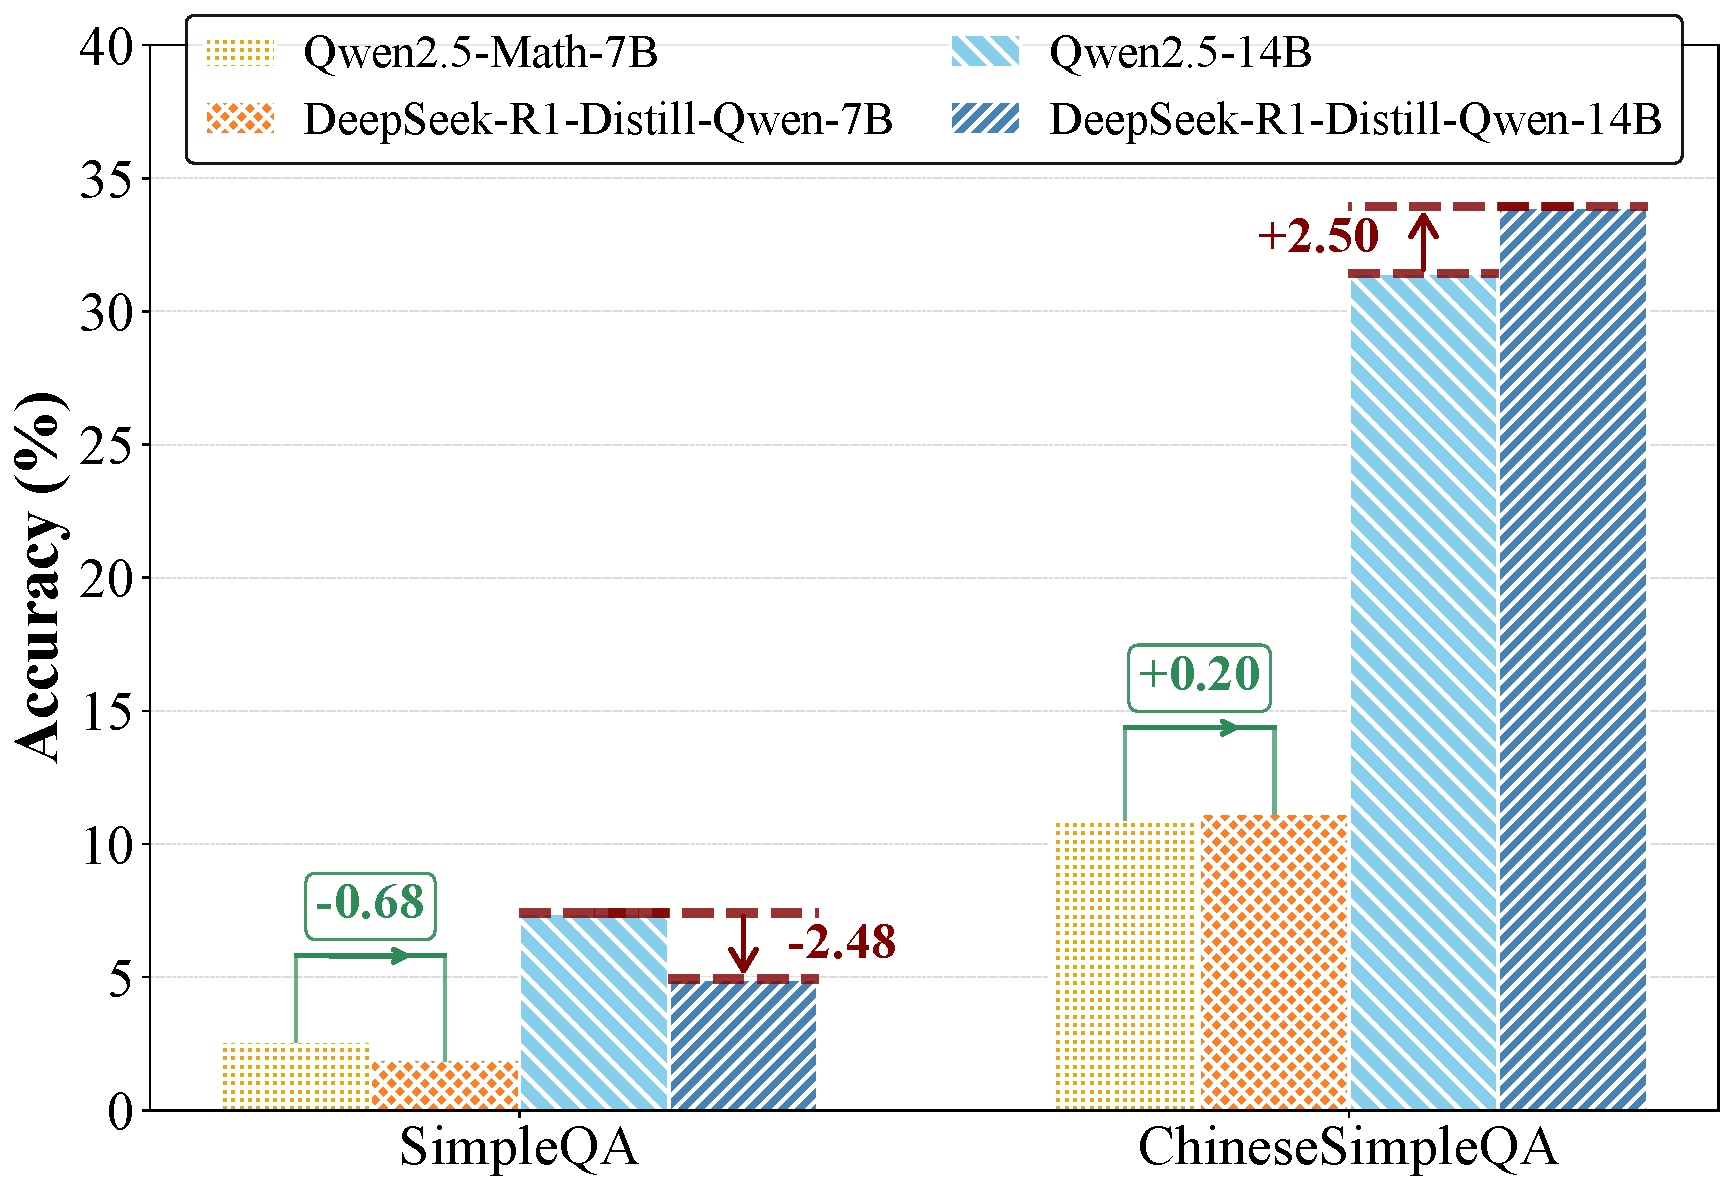
\includegraphics[width=\columnwidth]{images/model-comparison-barchart.pdf}
%     % \vspace{-2ex}
%     \caption{Performance of all models on SimpleQA and ChineseSimpleQA.}
%     \vspace{-3ex}
%     \label{slow-thinking-hallucination}
% \end{figure}
\begin{figure}[t!]
    \centering
    \resizebox{.45\textwidth}{!}{
    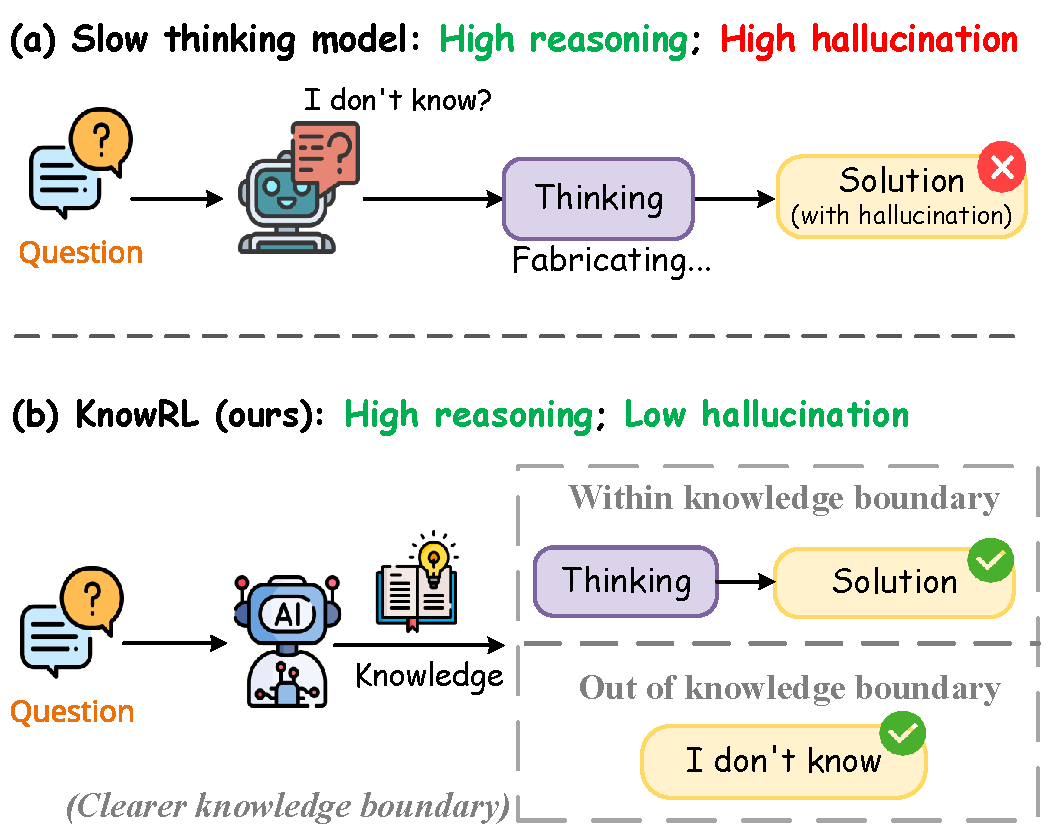
\includegraphics{images/intro.pdf}}
    \caption{KnowRL reduces hallucinations in slow-thinking models.}
     \vspace{-3ex}
    \label{fig:intro}
\end{figure}

The root cause lies in the way we currently train these models.
Standard RL heavily relies on outcome-oriented rewards, which optimize for the final answer while treating the reasoning process as a black box. 
This approach has two main flaws.
\textit{First}, it ignores the Knowledge Boundary---the model's ability to distinguish between what it knows and what it does not know. 
Without this boundary, models try to guess the answer to get the reward. 
\textit{Second}, it creates a supervision gap: model might generate a correct answer using wrong or made up reasoning steps. 
Since the reward signal depends solely on the final outcome, the model mistakenly learns that fabricating reasoning paths is a valid strategy; therefore, the RL algorithm unwittingly reinforces this hallucinated logic.
Consequently, the model becomes ``smart'' at reasoning but ``dishonest'' about facts.

Addressing this challenge with existing methods proves difficult. 
Retrieval Augmented Generation \citep[RAG;][]{lewis2020retrieval} faces significant retrieval efficiency bottlenecks when integrated into the extensive reasoning steps of slow thinking models. 
Supervised Fine Tuning \citep[SFT;][]{ouyang2022training} primarily relies on static knowledge injection. 
However, this paradigm suffers from severe catastrophic forgetting \citep{chen2025retaining}, often degrading the model's inherent reasoning capabilities. 
More fundamentally, SFT encourages the model to merely memorize static knowledge rather than learning the generalized behavior of reasoning.
Consequently, it fails to instill the critical strategy of ``knowing what you know and what you do not know''---a dynamic judgment of Knowledge Boundaries. 
In contrast, Reinforcement Learning is uniquely suited to shape this behavioral strategy \citep{gandhi2025cognitive}.
Therefore, there is an urgent need for a RL framework that can inherently instill factual discipline into the model's reasoning behaviors without compromising its reasoning capabilities.




% RL driven by outcome rewards often neglects the LLM's reasoning process, leading to correct outputs from flawed internal reasoning. 
% Generalizing such incorrect reasoning patterns significantly increases hallucination risk. 
% This issue is exacerbated in slow-thinking models trained via RL on mixed task types, partly because simple open-domain factual tasks and complex reasoning tasks (e.g., mathematics) have differing training requirements. 
% Fundamentally, models lacking factual guidance during training may resort to any means to obtain rewards, resulting in highly unreliable thinking processes. 
% Existing hallucination mitigation methods have limitations: Supervised Fine-Tuning \citep[SFT;][]{ouyang2022training} with high-quality data is costly and difficult to scale; Retrieval Augmented Generation \citep[RAG;][]{lewis2020retrieval} encounters efficiency and fusion challenges in long Chain-of-Thought (CoT) reasoning; and decoding-stage interventions \citep{chuang2023dola} can disrupt strategies learned through RL. 
% Crucially, these approaches do not consistently preserve strong reasoning capabilities while reducing hallucinations. 
% Therefore, a more reliable method involves introducing knowledge to supervise the model's thinking process during RL training.
\begin{figure}[t]
    \centering
    \resizebox{.45\textwidth}{!}{
    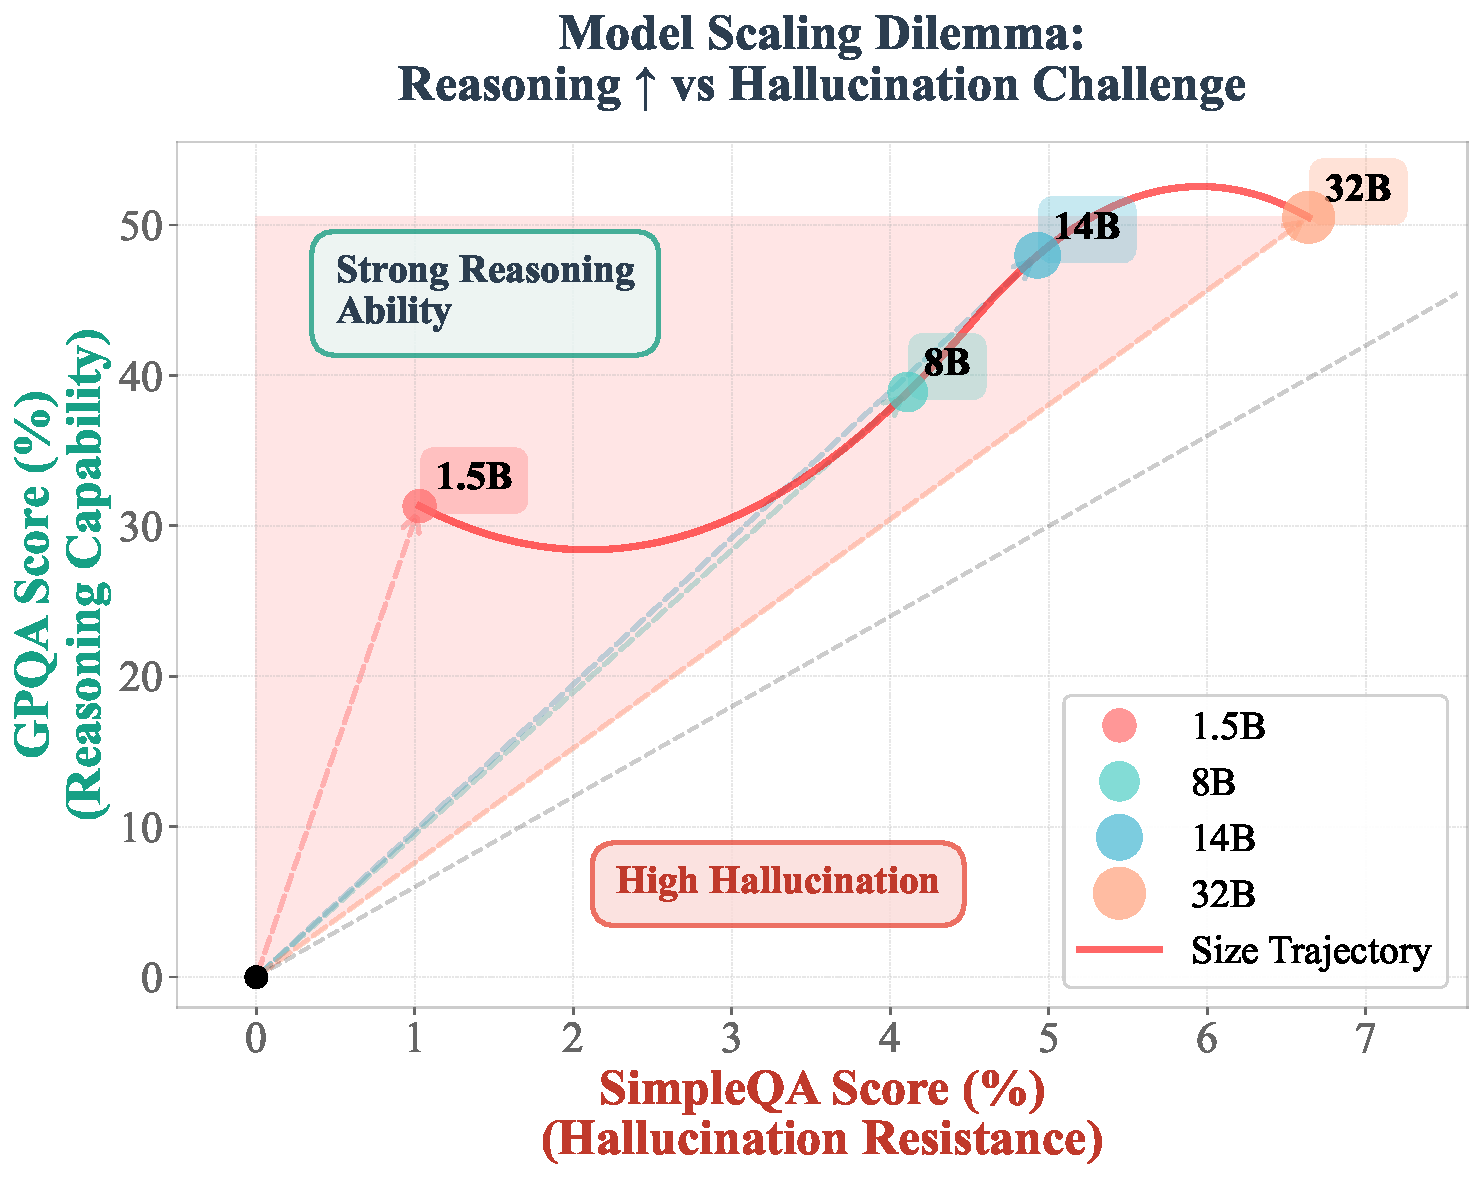
\includegraphics{images/model_scaling_analysis.pdf}}
    \caption{Scaling improves reasoning ability (GPQA) but does not reduce hallucinations (SimpleQA). Results are shown for DeepSeek-R1-Distill models of varying sizes (Qwen-1.5B, Llama-8B, Qwen-14B, Qwen-32B).}
    \vspace{-3ex}
    \label{fig:scaling}
\end{figure}

So, to bridge this gap, we propose Knowledge enhanced Reinforcement Learning (KnowRL), a framework that integrates factuality supervision directly into the RL reasoning loop. 
Unlike outcome-based approaches, KnowRL opens the ``black box'' of thinking. 
By decomposing the Chain of Thought into atomic facts and verifying them against the corresponding ground-truth knowledge, KnowRL provides dense, process level rewards. 
This design transforms the RL objective: instead of merely ``getting the answer right,'' the model is incentivized to reason faithfully and, crucially, to recognize its knowledge boundaries---learning to say ``I don't know'' rather than fabricating a plausible sounding response when information is missing, as illustrated in Figure~\ref{fig:intro}.

Experimental results validate the effectiveness of KnowRL. 
On hallucination benchmarks, KnowRL significantly reduces the error rate. 
For instance, dropping the Incorrect Rate on SimpleQA by 20.3\% for 7B slow thinking model. 
Crucially, this gain in factuality does not come at the cost of reasoning ability; KnowRL maintains strong performance on complex reasoning datasets like GPQA and AIME 2025. 
Furthermore, our method demonstrates strong transferability and Out-Of-Distribution (OOD) generalization to knowledge domains outside the training distribution; it significantly improves performance on ChineseSimpleQA~\citep{he2024chinese} even when the primary knowledge source is purely English-based. 
These findings suggest that KnowRL helps the model internalize a universal verification behavior rather than merely memorizing language-specific facts.  
These results confirm that KnowRL successfully aligns the slow thinking process with factual accuracy, offering a robust path for building reliable reasoning models.

% To address this, we propose Knowledge-enhanced Reinforcement Learning (KnowRL), a method that integrates a factuality reward into the RL training process. This reward, inspired by FactScore \citep{min2023factscore} and obtained by evaluating textual support against an external knowledge base, guides the model to perform fact-based slow thinking. 
% KnowRL cooperatively optimizes reasoning and fact-following in slow-thinking models by helping them learn better knowledge boundaries to avoid fabricating facts, as illustrated in Figure~\ref{fig:intro}. 
% Our extensive experiments validate KnowRL's significant impact. 
% Across benchmarks such as TruthfulQA~\citep{lin2021truthfulqa}, KnowRL consistently mitigates hallucinations while preserving reasoning ability. For distillation-based slow-thinking models, KnowRL training reduces the error rate on SimpleQA by 20.3\%, while maintaining strong reasoning performance on GPQA~\citep{rein2024gpqa} and AIME 2025. Moreover, KnowRL substantially decreases incorrect responses on ChineseSimpleQA~\citep{he2024chinese}, a dataset outside our English-based knowledge source, demonstrating that KnowRL learns transferable knowledge boundaries and improves factual reliability beyond the original knowledge base.




% The main contributions of this paper are as follows:
% \begin{itemize}
%     \item We introduce KnowRL, a novel framework using factuality rewards from external knowledge to reduce hallucinations in LLMs while preserving their reasoning ability.
%     \item We demonstrate through comprehensive experiments that KnowRL effectively mitigates hallucinations and maintains reasoning in diverse slow-thinking models.
%     \item We contribute a carefully constructed, high-quality training dataset for factual tasks, crucial for initializing and training KnowRL.
% \end{itemize}

% \begin{itemize}
%     \item We propose KnowRL, a Reinforcement Learning framework using factuality rewards from knowledge verification to reduce slow-thinking model hallucinations while maintaining strong reasoning ability.
%     % \item Our experiments identify optimal KnowRL training configurations: essential cold-start SFT for factuality reward efficacy, and balanced cold-start data volume and RL training duration to mitigate hallucinations without impairing reasoning or causing overtraining.
%     \item Our experimental analyses identify key training configurations for KnowRL's efficacy: foundational cold-start SFT is essential for activating factuality rewards, while optimal cold-start data volume and RL training duration are crucial to balance hallucination mitigation with reasoning ability, preventing negative impacts from suboptimal data quantities or overtraining.
%     \item We constructed high-quality reasoning training datasets for open-domain factual tasks and distilled high-quality SFT long COT datasets for factual tasks.
% \end{itemize}





%



\section{Hallucination in Slow-thinking Models}

% \begin{tcolorbox}[colback=gray!5,colframe=gray!40!black,title=Definition]
% \textbf{Slow-thinking models} refer to language models that solve tasks via explicit multi-step reasoning. 
% This design enhances their ability to decompose complex problems but simultaneously increases exposure to factual errors, as inaccuracies may propagate across reasoning steps.
% \end{tcolorbox}


While slow-thinking models provide structured reasoning, they also amplify the risk of hallucinations. 
Figure~\ref{fig:scaling} illustrates this trade-off: larger DeepSeek-R1-Distill models achieve higher GPQA scores (reasoning ability) but fail to improve on SimpleQA (hallucination resistance), showing that scaling strengthens reasoning without resolving factual reliability issues.

\begin{definitionbox}
\textbf{The Hallucination Challenge in Slow-Thinking Models.} The multi-step reasoning of slow-thinking models creates a critical vulnerability to error propagation, where an initial factual inaccuracy cascades through the reasoning chain to yield a conclusion that is logically coherent but factually ungrounded.
\end{definitionbox}

The root cause lies in the factual supervision gap within current training paradigms. Existing approaches often emphasize reproducing reasoning patterns or final outcomes without verifying the factual accuracy of intermediate reasoning steps, leading models to generate coherent yet factually unsupported chains of thought.
Consequently, models may generate reasoning chains that sound coherent but are factually ungrounded, as evidenced by prior work \citep{heyman2025reasoning,patel2024multi,arcuschin2025chain}. 

This gap also explains why outcome-based RL is insufficient: rewarding only final correctness neglects factual consistency during reasoning. 
Worse, it may reinforce “lucky” but unreliable chains. 
Thus, mitigating hallucinations in slow-thinking models requires training strategies that directly enforce factual grounding—an objective we address with KnowRL.

% We use SimpleQA, TruthfulQA and ChineseSimpleQA datasets as the hallucination evaluation datasets, and GPQA dataset as the dataset for evaluating the model's reasoning ability. 



% \begin{figure}[h]
%     \centering
%     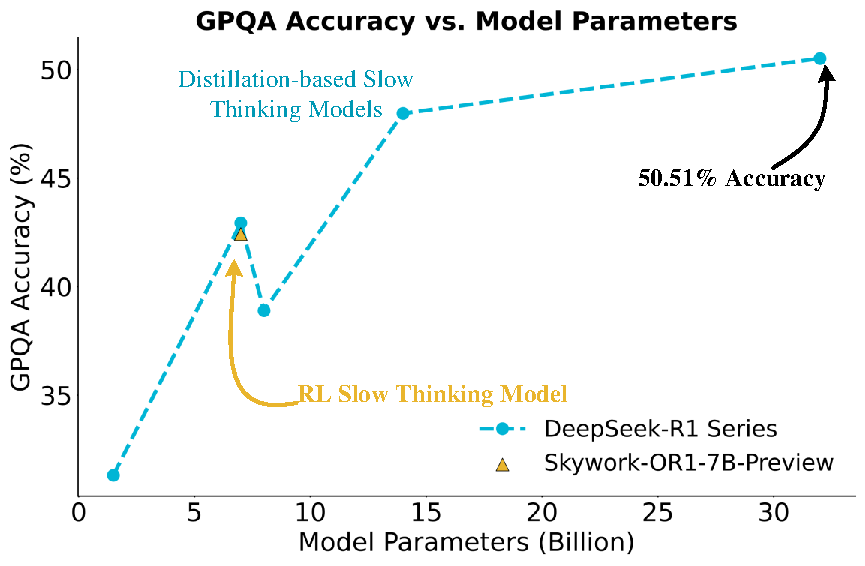
\includegraphics[width=\columnwidth]{images/slow-thinking.pdf}
%     % \vspace{-2ex}
%     \caption{Accuracy of the slow thinking model on the GPQA dataset.}
%     \vspace{-3ex}
%     \label{slow-thinking-gpqa}
% \end{figure}






%\section{Data Construction} %%%%%%%%%%%%%%%%%%%%%

In large-scale training, redundant information increases storage and computation costs and affects the performance of RL training. 
To ensure the quality of the training data for RL, we screen high-quality Q\&A data from several open-source datasets for training and use DeepSeek-R1 to obtain long COT data for SFT. The following are data construction steps.

\subsection{RL Data Construction}
 We use part of the data extracted from NqOpen \cite{kwiatkowski2019natural,lee2019latent}, WebQuestions \citep{berant2013semantic}, and ComplexQuestions \citep{bao2016constraint} as factual question data sources.

\paragraph{Pre-processing and Simple Filtering.}
First of all, we filter out data that has multiple possible answers. 
This is because data with non-unique answers can easily lead to unstable training. 
At the same time, we filtered out the data with no obvious questioning tone in the questions, as such data can easily lead to the model not knowing the meaning of the question and thus blindly exploring it during the training process, thus affecting the training performance. 
We believe that there is no need for RL training for simple questions, so we use the Qwen2.5-7B-Instruct \citep{qwen2.5} to filter the simple data in the data source, and the filtering method is to filter out the questions that are answered correctly for the first time by the Qwen2.5-7B-Instruct.

\paragraph{Multiple De-duplication and Entropy Filtering.}
We decided to de-duplicate the data of NqOpen due to its large amount and not strictly filtered and cleaned. 
We use Semhash \citep{minishlab2025semhash} to perform exact de-duplication and semantic de-duplication on the data of NqOpen after filtering in step 1 to ensure data diversity. 
Exact de-duplication means excluding duplicate data in the dataset with exactly the same problem.
We use potion-base-8M \citep{minishlab2024model2vec} as the sentence embedding model for semantic de-duplication.
Based on the generated semantic vectors, we use the approximate nearest neighbor search algorithm to quickly search for similar vectors, mark the data with cosine similarity greater than a threshold as similar data and form a cluster, only one sample is selected from a cluster, and the rest of the data are marked as duplicate data and filtered. 
According to the entropy value calculated for each problem, the top 80\% proportion of data is selected as the filtered data, thus ensuring data diversity. 
Finally, the data from NqOpen after de-duplication and the filtered WebQuestions and ComplexQuestions data obtained in step 1 are combined to form the two-stage filtered data.

\paragraph{Refinement and Entity Extraction.}
In this step, we use the GPT-4O and predefined rules to check each question of the data obtained in step 2, to exclude questions that are not formal, do not have enough information to support reasoning about the answer, and are not formal in language. 
Carefully designed prompts enable the GPT-4O to accept or reject each data item, and for accepted items, to normalize, correct, and extract entities. 
Appendix shows the prompts used by the GPT-4O model for data filtering.

\paragraph{Difficulty Filtering.}
To avoid excessive difficulty in the training data, we choose to further filter the data obtained from the previous step using DeepSeek-R1, specifically selecting questions that DeepSeek-R1 answers correctly on its first attempt. 
This step also helped us get the long COT data needed for the SFT baseline.

\paragraph{Wikipedia-grounded Data Filtering.}
The goal of this step is to filter out data that cannot be matched to the corresponding knowledge from the Wikipedia knowledge source.
We use Wikipedia\footnote{20231101.en, \url{https://dumps.wikimedia.org/}.} (6.4 million entries) as our knowledge source. 
Based on each data item's entities, we retrieve corresponding Wikipedia entries and add their textual content as knowledge for the item into our knowledge base. An entity must exactly match a Wikipedia entry or be fully contained within a Wikipedia entry title for the match to be successful. 
To avoid redundancy, each entity keyword links to no more than three Wikipedia entries. 
Data items containing entities that do not match any Wikipedia entry are filtered out in this paper. 
Additionally, to ensure the stability of SFT training, we choose to retain only the 3,177 data items where DeepSeek-R1's output length is between 300 and 700 tokens as training data. 
So, We complete the filtering and construction of the training data.

\subsection{ColdStart Data Construction}
We obtain another part of the remaining data from NqOpen and perform the same filtering steps as we did to construct the RL training data.
We use DeepSeek-R1 to distill the long COT data and filter out the questions that DeepSeek-R1 answered correctly the first time. 
And merge the data that failed to match the knowledge in the RL training data construct as data source. 
Only 1798 data items with DeepSeek-R1 output length between 300 and 700 are kept as cold-start training data.





%\section{Preliminary}

In this paper, we chose to first use supervised fine-tuning for cold-start training of slow thinking models and then use the Grouped Relative Policy Optimization \citep[GRPO;][]{shao2024deepseekmath}) algorithm for reinforcement learning training. We will introduce SFT and reinforcement learning algorithms for language model fine-tuning.

SFT is a method for improving the ability of a model to follow instructions and adapt to specific downstream tasks by having the model parameters fit a high-quality dataset.
SFT aims to minimize the negative log-likelihood loss to maximize the conditional probability \( P_{\theta}(y|x) \) of generating the target sequence \( y \) given the input \( x \). For the entire dataset \( D \), the loss function \( L_{SFT} \) of SFT can be expressed as:
\begin{equation}
L_{SFT}(\theta) = -\sum_{(x,y) \in D} \log P_{\theta}(y|x).
\end{equation}
As \( L_{SFT} \) decreases continuously, the probability of the model generating the expected output given the input gradually increases. Using SFT as a cold-start training before reinforcement learning training can speed up the convergence of the reward curve during reinforcement learning training.

GRPO is a highly efficient reinforcement learning method that replaces traditional value network-based advantage estimation with a unique group relative reward mechanism. GRPO removes the value network found in traditional Proximal Policy Optimization \citep[PPO;][]{schulman2017proximal}, retaining only the policy network. This, to a certain extent, reduces computational and memory requirements.

The group relative reward mechanism in GRPO refers to sampling multiple candidate outputs (or actions) from the current prompt (or state) to form a "response group" (or action group). Then, by normalizing the rewards of the outputs within the group, a relative advantage value is obtained, thereby replacing traditional absolute advantage estimation. The GRPO objective function is constructed from two main components per timestep $t$.
First, the PPO-style clipped surrogate objective is defined as:
\begin{equation} \label{eq:grpo_clip}
L^{\text{CLIP}}_t(\theta) = \min(r_t(\theta)A_t, \text{clip}(r_t(\theta), 1-\epsilon, 1+\epsilon)A_t).
\end{equation}
Second, the gradient regularization term introduced by GRPO is:
\begin{equation} \label{eq:grpo_reg}
L^{\text{REG}}_t(\theta) = \lambda \|\nabla_\theta r_t(\theta)\|^2.
\end{equation}
The overall GRPO objective function, $L^{\text{GRPO}}(\theta)$, is then the expectation over timesteps $t$ of the difference between these two components:
\begin{equation} \label{eq:grpo_objective_final}
L^{\text{GRPO}}(\theta) = \mathbb{E}_t [L^{\text{CLIP}}_t(\theta) - L^{\text{REG}}_t(\theta)].
\end{equation}

The GRPO objective function, $L^{\text{GRPO}}(\theta)$ as defined in Equation~\eqref{eq:grpo_objective_final}, aims to improve the policy by optimizing the policy parameters $\theta$. It is an expectation over timesteps $t$.
The first component for each timestep, $L^{\text{CLIP}}_t(\theta)$ given by Equation~\eqref{eq:grpo_clip}, is the classic clipped surrogate objective from PPO. Within this term, $r_t(\theta)$ is the policy probability ratio, specifically $\frac{\pi_\theta(a_t|s_t)}{\pi_{\text{old}}(a_t|s_t)}$, which compares the probability of taking action $a_t$ in state $s_t$ under the current policy $\pi_\theta$ (determined by parameters $\theta$) versus the old policy $\pi_{\text{old}}$ (used to collect the data). $A_t$ represents the advantage function, which in GRPO specifically refers to the relative advantage value calculated via the group relative reward mechanism, quantifying how good the current action is. The $\text{clip}$ function constrains $r_t(\theta)$ to the range $[1-\epsilon, 1+\epsilon]$, where $\epsilon$ is a small hyperparameter used to limit the magnitude of policy updates, preventing excessively large updates that could destabilize training.
The second component for each timestep, $L^{\text{REG}}_t(\theta)$ from Equation~\eqref{eq:grpo_reg}, is the gradient regularization term introduced by GRPO. Here, $\nabla_\theta r_t(\theta)$ denotes the gradient of the policy probability ratio $r_t(\theta)$ with respect to the policy parameters $\theta$, and $\lambda$ is a regularization coefficient. This term, $L^{\text{REG}}_t(\theta)$, penalizes the L2 norm (squared) of the gradient of the policy probability ratio, further constraining the magnitude of policy updates. This helps prevent overly rapid policy changes and ensuing instability, which is particularly important for GRPO as it operates without the assistance of a value network. The final objective $L^{\text{GRPO}}(\theta)$ then combines these by taking the expectation of $L^{\text{CLIP}}_t(\theta) - L^{\text{REG}}_t(\theta)$.









\begin{figure*}[t!]
    \centering
    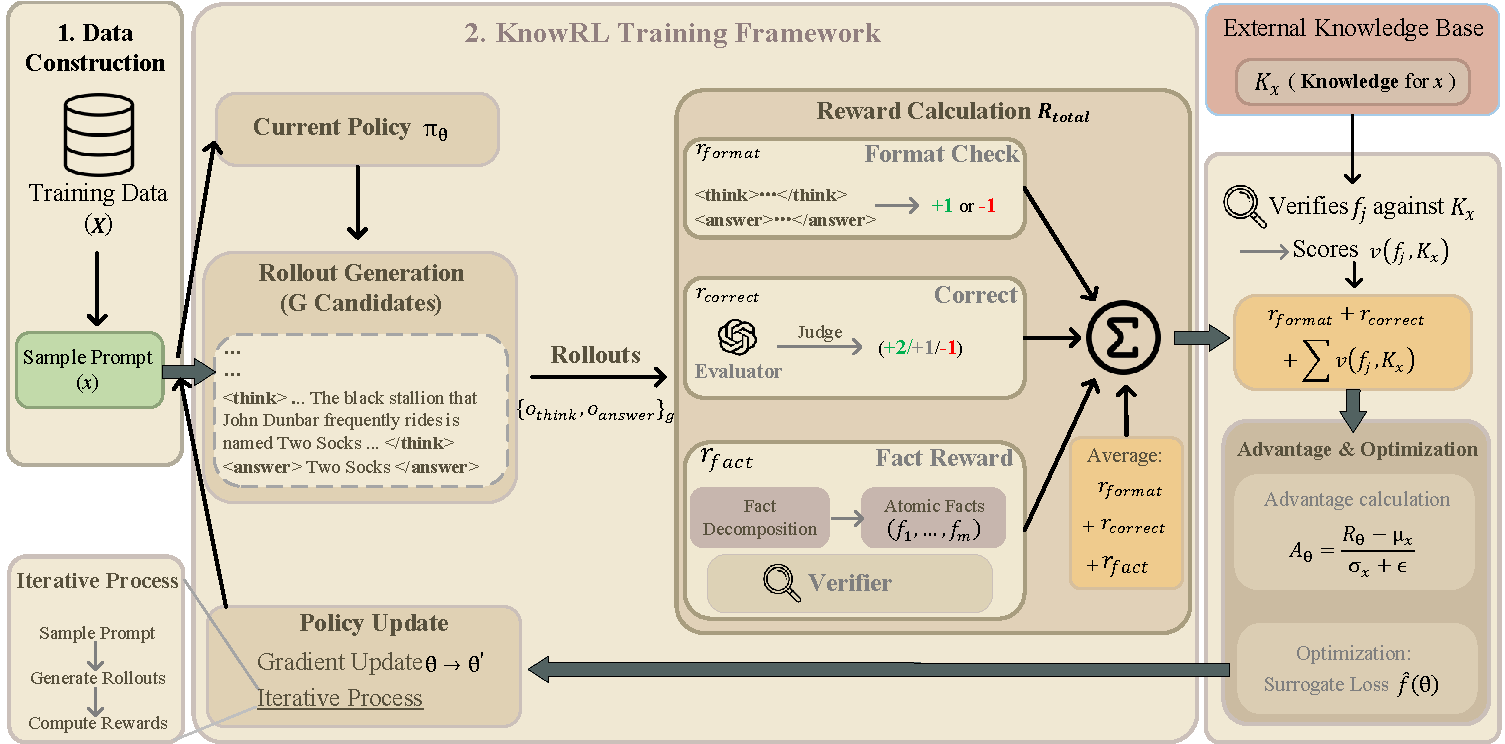
\includegraphics[width=1.0\linewidth]{images/framework1.pdf}
    % \vspace{-2ex}
    \caption{\textbf{Overview of the KnowRL framework.} We first construct training data matched with external knowledge. During RL training, we decompose the generated reasoning process into atomic facts and verify them against the knowledge base. Finally, we optimize the model using a composite reward that combines these factual scores with correctness and format checks.}
    % \vspace{-3ex}
    \label{knowrl}
\end{figure*}

\section{Knowledgeable Reinforcement Learning}

To address the high hallucination rates in slow-thinking models, we propose a fundamental shift in supervision: focusing on the \textbf{\textit{reasoning process}} rather than only on final outcomes. 
To this end, we introduce \texttt{KnowRL}, a Knowledge enhanced Reinforcement Learning framework designed to guide models toward verifiable and boundary-aware reasoning by integrating factual supervision directly into the RL loop. 
As illustrated in Figure~\ref{knowrl}, we first construct training data matched with knowledge, and then conduct RL training using a composite reward that balances factual correctness with reasoning quality (details in Appendix~\ref{appendix:data-construction}). 
By enforcing factual consistency at the step level, KnowRL effectively corrects incorrect reasoning paths and encourages models to recognize their \textbf{\textit{knowledge boundaries}}, ultimately leading to a more faithful and self-aware thinking process.





KnowRL builds upon the Group Relative Policy Optimization (GRPO) algorithm by introducing \emph{factuality supervision} into the CoT reasoning process. This integration ensures that the model is guided not just by the final answer, but by the factual accuracy of its thinking steps. In the following, we detail how we design the composite Reward Function to evaluate these steps and how we implement the Factuality-Guided Policy Optimization.

\medskip
\noindent\textbf{Reward Function.}  
Given a rollout \(o=(o_{\mathrm{think}},o_{\mathrm{answer}})\), inspired by FactScore~\citep{min2023factscore}, we use GPT-4o-mini for the factual verification process. 
We decompose the reasoning trace into \(M\) atomic facts \(\Phi(o_{\mathrm{think}})=\{f_1,\dots,f_M\}\). 
Given an external knowledge base $K$, each atomic fact $f_j$ is checked against its most relevant knowledge set $K_x \subseteq K$\footnote{Retrieved using \texttt{sentence-transformers/gtr-t5-large}.} to obtain a verification score $v(f_j, K_x) \in \{0,1\}$.
The factuality reward is then defined as the proportion of supported facts:
\begin{equation}
\label{eq:factual-score}
r_{\mathrm{fact}}(o)=
\begin{cases}
\displaystyle \frac{1}{M}\sum_{j=1}^{M}v(f_j,K_x), & M>0,\\[6pt]
0, & M=0 .
\end{cases}
\end{equation}

Additional components include a \emph{\textbf{format reward}} \(r_{\mathrm{format}}(o)\) and a \emph{\textbf{correct reward}} \(r_{\mathrm{correct}}(o)\). 
The format reward verifies whether the output follows the required \texttt{<think>...</think><answer>...</answer>} structure: if the format is valid, \(r_{\mathrm{format}}(o)=+1\); otherwise, \(r_{\mathrm{format}}(o)=-1\). 
The correctness reward evaluates the final answer \(o_{\mathrm{answer}}\) using an evaluator model (GPT-4o-mini): if the answer is correct, \(r_{\mathrm{correct}}(o)=+2\); if the model explicitly refuses, \(r_{\mathrm{correct}}(o)=+1\); if the answer is incorrect, \(r_{\mathrm{correct}}(o)=-1\). 
The composite reward is then defined as
\begin{equation}
R_{\mathrm{total}}(o) = r_{\mathrm{format}}(o) + r_{\mathrm{correct}}(o) + r_{\mathrm{fact}}(o).
\end{equation}




\medskip
%\noindent\textbf{Factuality-Aware GRPO Training.}\;

\noindent\textbf{Factuality–Guided Policy Optimisation.}\;
For every prompt $x$ the current policy
$\pi_{\theta_{\text{old}}}$ generates a \emph{group} of $G$ candidate
roll-outs
$\{o^{(g)}\}_{g=1}^{G}\!\sim\!\pi_{\theta_{\text{old}}}(\cdot|x)$, where
$G$ is the group size. 
Each trajectory is scored by the composite reward
$R_{\mathrm{total}}(\cdot)$, yielding a set of scalars
$\mathcal{R}_x=\{R_g\}_{g=1}^{G}$.

\noindent\textbf{Advantage construction.}
We summarise $\mathcal{R}_x$ with its sample mean
$\mu_{x}$ and standard deviation $\sigma_{x}$. 
The credit assigned to trajectory $g$ is the
\emph{group-relative advantage}
\begin{equation}
\label{eq:adv}
A_{g}\;=\;\frac{R_{g}-\mu_{x}}{\sigma_{x}+\varepsilon},
\end{equation}
where $\varepsilon\!(\!\ll\!1)$ avoids division by~zero.
$A_{g}$ is positive if $o^{(g)}$ attains above-average factual reward and negative otherwise, turning factual supervision into a signed learning signal.

\noindent\textbf{Likelihood ratio.}
Define the trajectory-level importance ratio
\[
\varrho_{g}
=\frac{\pi_{\theta}\!\bigl(o^{(g)}\!\mid x\bigr)}
       {\pi_{\theta_{\mathrm{old}}}\!\bigl(o^{(g)}\!\mid x\bigr)}.
\]
The pair $(\varrho_{g},A_{g})$ fully characterises how $o^{(g)}$ should
influence the update: \emph{increase} its probability if
$\varrho_{g}A_{g}>0$ and \emph{decrease} otherwise.

\noindent\textbf{Surrogate objective.}
Using these short symbols enables a compact, column-friendly surrogate:
\begin{equation}
\label{eq:surrogate}
\hat{\mathcal{J}}(\theta)=
\frac{1}{G}\sum_{g=1}^{G}
\min\!\bigl(
      \varrho_{g}A_{g},\,
      \operatorname{clip}(\varrho_{g},1-\epsilon,1+\epsilon)A_{g}
     \bigr),
\end{equation}
with a small clip threshold $\epsilon$ to bound the update.
Because $A_{g}$ encodes factual advantage,
maximising $\hat{\mathcal{J}}$ explicitly transfers probability mass from hallucination-heavy traces ($A_{g}<0$) to trajectories whose CoT is knowledge-supported ($A_{g}>0$).


\noindent\textbf{Regularised loss.}\;
To preserve exploration and limit divergence from the frozen reference policy $\pi_{\text{ref}}$, we add (i) an entropy bonus and (ii) a KL anchor.  
Let $o$ denote a complete rollout and $o_t$ its $t$-th token.  
The token-level Shannon entropy on prompt $x$ is therefore
$\mathcal{H}(\pi_{\theta}(\cdot|x))
      =-\sum_{t}\pi_{\theta}(o_t|x)\log\pi_{\theta}(o_t|x)$.
Its mini-batch expectation and the corresponding KL expectation are
$\mathcal{E}_{\mathcal{H}}\triangleq\mathbb{E}_{x}[\mathcal{H}(\pi_{\theta}(\cdot|x))]$ and
$\mathcal{E}_{\mathrm{KL}}\triangleq\mathbb{E}_{x}[D_{\mathrm{KL}}(\pi_{\theta}(\cdot|x)\|\pi_{\text{ref}}(\cdot|x)]$.
With scalar weights $\beta_{\mathcal{H}},\beta_{\mathrm{KL}}>0$, the final objective becomes
\begin{equation}
\label{eq:loss}
\mathcal{L}_{\text{KnowRL}}
  = -\hat{\mathcal{J}}(\theta)
    \;+\;\beta_{\mathcal{H}}\mathcal{E}_{\mathcal{H}}
    \;+\;\beta_{\mathrm{KL}}\mathcal{E}_{\mathrm{KL}}.
\end{equation}


During training, each gradient step proceeds as follows.  
First, a mini-batch of prompts $x$ is sampled and the old policy
$\pi_{\theta_{\mathrm{old}}}$ produces a group $\mathcal{O}_x$ of
$G$ roll-outs.
Next, every trajectory $o^{(g)}\!\in\!\mathcal{O}_x$ undergoes the
knowledge check that yields the composite reward
$R_g=R_{\mathrm{total}}(o^{(g)})$, whose factual component
$r_{\text{fact}}$ is computed against the external knowledge base.
The set $\{R_g\}$ is then converted into group-relative advantages
$A_g$ via Eq.\,\eqref{eq:adv}, so that a higher proportion of verified
facts directly translates into a larger positive $A_g$, whereas
hallucinated chains of thought receive negative credit.
The new policy $\pi_{\theta}$ is updated by maximising the factual
surrogate $\hat{\mathcal{J}}(\theta)$ in Eq.\,\eqref{eq:surrogate}
while minimising the regularised loss
$\mathcal{L}_{\text{KnowRL}}$ in Eq.\,\eqref{eq:loss};
this couples the likelihood ratio $\varrho_g$ with $A_g$ so that
gradients \emph{increase} the probability of
knowledge supported reasoning and \emph{decrease} that of
hallucination prone trajectories.  
Iterating this loop prompt sampling, factual verification,
advantage normalisation, and loss-driven update---yields a policy that
systematically suppresses hallucinations yet preserves answer accuracy.




% KnowRL is a factuality supervised variant of GRPO. By rewarding the proportion of correct atomic facts in chain-of-thought and integrating entropy-aware regularization, it encourages models to \emph{think factually} while maintaining exploration, effectively mitigating hallucinations in slow-thinking models.










































% \subsection{Reward Function Design}
% We design a special reward function to guide the model in generating outputs that are not only factual in the reasoning process but also provide accurate final answers. 
% The final reward for a model output \(o\) is denoted as \(R_{\text{total}}(o)\).

% \paragraph{Format Reward.}
% The format reward is to justify the specific \texttt{<think>}$o_{\text{think}}$\texttt{</think>} and \texttt{<answer>}$o_{\text{answer}}$\texttt{</answer>} structure, where \(o_{\text{think}}\) denote the thinking process and \(o_{\text{answer}}\) denote the final answer.
% \begin{equation}
% \label{eq:reward_format}
% R_{\text{format}}(o) = \begin{cases} +1 & \text{if } o \text{ has valid format} \\ -1 & \text{otherwise} \end{cases}.
% \end{equation}

% \paragraph{Correct Reward.}
% The correct reward evaluates the accuracy of the final answer \(o_{\text{answer}}\), which is assessed by the GPT-4o-mini. 
% A model's response can be correct, incorrect, or a refusal, and as shown in~\eqref{eq:reward_correct}, both incorrect answers and refusals receive -1 penalty from the correctness reward component.
% \begin{equation}
% \label{eq:reward_correct}
% R_{\text{correct}}(o) = \begin{cases} +2 & \text{if } o_{\text{answer}} \text{ is correct} \\ -1 & \text{otherwise} \end{cases}.
% \end{equation}

% \paragraph{Fact Reward.}
% The fact reward quantifies the factuality of the reasoning process articulated in \(o_{\text{think}}\). 
% We achieve this by using FactScore, which decomposes \(o_{\text{think}}\) into atomic facts and verifies their support against an external knowledge base \(K\). 
% We use the Wikipedia text matched with each entry in the training data to construct \(K\). 
% We first utilize GPT-4o-mini to decompose the input text into several atomic facts. 
% Subsequently, we use an NLI model\footnote{The DeBERTa-v3-base-mnli-fever-anli model.} to determine if each atomic fact is supported by text retrieved from the \(K\). 
% \(N_{\text{supported}}(o_{\text{think}}, K)\) is the number of atomic facts in \(o_{\text{think}}\) supported by \(K\). 
% \begin{equation}
% \label{eq:reward_fact}
% R_{\text{fact}}(o) = \min\left(\frac{N_{\text{supported}}(o_{\text{think}}, K)}{15}, 1.0\right).
% \end{equation}
% This encourages the model to ground its reasoning in verifiable facts.

% The \(R_{\text{combined}}(o)\) is then formulated to avoid excessively penalizing factual reasoning when the final answer is incorrect:
% \begin{equation}
% \label{eq:reward_combined}
% \resizebox{0.9\hsize}{!}{$
% R_{\text{combined}}(o) = \begin{cases} 
%   +2 & \text{if } o_{\text{answer}} \text{ is correct} \\ 
%   -1 + R_{\text{fact}}(o) & \text{if } o_{\text{answer}} \text{ is incorrect} 
% \end{cases}$}.
% \end{equation}
% This ensures that even if an answer is marked incorrect, the model can still receive a relatively positive reward based on the factuality of its thought.
% % Given that all weights (\(w_{\text{format}}, w_{\text{combined}}\)) are set to 1.0
% Finally, the total reward is defined as:
% \begin{equation}
% \label{eq:reward_total}
% R_{\text{total}}(o) = R_{\text{format}}(o) + R_{\text{combined}}(o).
% \end{equation}


% \subsection{RL Training.}
% We first cold-start the model with SFT to establish a more stable foundation for RL training. For the subsequent RL stage, we employ the Group Relative Policy Optimization \citep[GRPO;][]{shao2024deepseekmath} algorithm on our own constructed dataset. The GRPO process optimizes the model's policy using a combination of a correct reward and our designed fact reward. This fact-based reward guidance is crucial, as it teaches the model to ground its reasoning in facts, thereby effectively mitigating hallucination while maintaining or enhancing its reasoning capabilities\footnote{Qwen3 \citep{yang2025qwen3} is also trained through RL with multiple reward combinations. In the same period, we independently propose KnowRL and construct our own training data for factual tasks. We will open source our training data and code.}.

%We briefly introduce it in the following:

% \paragraph{Group Relative Rewards and Advantage ($A_t$).}
% The model first generates multiple candidate inference paths (actions $o_t$) for a given input cue $q_t$ based on the current policy $\pi_\theta$, forming a “response group”.
% We will then evaluate each path using the reward function $R_{\text{total}}(o_t)$. 
% Then, GRPO normalizes these rewards within the group to get a relative advantage $A_t$ for each response. 
% This value-network-free approach quantifies how well a response performed compared to others generated by the same policy for the same input.

% The GRPO method consists of two key components: a clipped policy optimization term that stabilizes training by constraining policy updates, and a gradient regularization term that controls update magnitudes. Together, they optimize the policy model while ensuring reliable reasoning generation—all without requiring a value network.

% \paragraph{Clipped Surrogate Objective.}
% The GRPO objective function aims to improve the policy $\pi_\theta$ by optimizing its parameters $\theta$. 
% The first component for each timestep $t$ is the PPO-style clipped surrogate objective $L^{\text{CLIP}}_t(\theta)$:
% \begin{equation}
% \label{eq:paper_grpo_clip}
% \resizebox{0.95\hsize}{!}{$
% L^{\text{CLIP}}_t(\theta) 
% = \min(r_t(\theta)A_t, \text{clip}(r_t(\theta), 1-\epsilon, 1+\epsilon)A_t).$}
% \end{equation}
% where $r_t(\theta) = \frac{\pi_\theta(a_t|s_t)}{\pi_{\theta_{\text{old}}}(a_t|s_t)}$ is the policy probability ratio, comparing the probability of generating the reasoning path $a_t$ under the current policy $\pi_\theta$ versus the old policy $\pi_{\theta_{\text{old}}}$. 
% $A_t$ is the relative advantage calculated as described above. 
% The $\text{clip}$ function, with a small hyperparameter $\epsilon$, constrains $r_t(\theta)$ to the range $[1-\epsilon, 1+\epsilon]$, ensuring stable updates for learning complex reasoning and factual adherence.

% \paragraph{Gradient Regularization.}
% The second component for each timestep $t$ is the gradient regularization term $L^{\text{REG}}_t(\theta)$ introduced by GRPO:
% \begin{equation} \label{eq:paper_grpo_reg}
% L^{\text{REG}}_t(\theta) = \lambda \|\nabla_\theta r_t(\theta)\|^2.
% \end{equation}
% where $\lambda$ is a regularization coefficient that penalizes large gradients of the policy probability ratio $r_t(\theta)$ with respect to the policy parameters $\theta$. 
% This further constrains the magnitude of policy updates, which is particularly important for GRPO's stability as it operates without a value network.

% The final GRPO objective $L^{\text{GRPO}}(\theta)$ combines these components by taking the expectation over timesteps $t$:
% \begin{equation} \label{eq:paper_grpo_objective}
% L^{\text{GRPO}}(\theta) = \mathbb{E}_t[L^{\text{CLIP}}_t(\theta) - L^{\text{REG}}_t(\theta)].
% \end{equation}
% By optimizing this objective, GRPO guides slow-thinking models to discover and reinforce policies that produce reasoning paths that are not only correct but also fact-based. 


% \begin{table*}[!htbp]
%     \centering
%     \small
%     \setlength{\tabcolsep}{3.2pt}
%     \renewcommand{\arraystretch}{1.2} % Slightly increase row height for readability
%     \begin{tabular}{l|ccc|cc}
%     \toprule
%     \multirow{2}{*}{\makecell[c]{\normalsize\textbf{KnowRL}}} & \multicolumn{3}{c|}{\textbf{Hallucination}} & \multicolumn{2}{c}{\textbf{Reasoning}} \\
%     \cmidrule(lr){2-4} \cmidrule(lr){5-6}
%     & \small\textbf{TruthfulQA} & \small\textbf{SimpleQA} & \small\textbf{ChineseSimpleQA}  & 
%     \small\textbf{GPQA} & \small\textbf{AIME 2025}\\
   
%     \midrule
%     \multicolumn{6}{c}{\textbf{DeepSeek-R1-Distill-Qwen-7B}} \\
%     \text{allbehavior}           & 37.58 & 2.88 & 10.47  & 38.38 & 10.00  \\
%     \text{0.25nobehavior}        & 36.96 & 3.83 & 13.57  & 35.35 & 20.00  \\
%     \text{0.5nobehavior}         & 37.21 & 3.94 & 13.47  & 37.37 & 23.33  \\
%     \text{0.75nobehavior}        & 35.86 & 3.74 & 12.03  & 34.34 & 16.67  \\
%     \text{nobehavior}            & 36.23 & 3.54 & 12.63  & 34.34 & 16.67  \\
%     \bottomrule
%     \end{tabular}
%     \vspace{-1ex}
%     \caption{ Main Experiment}
%     \vspace{-3ex}
%     \label{tab:tofu}
% \end{table*}


\begin{table}[t]
    \centering
    \small
    \begin{tabular}{llc}
    \toprule
    \textbf{Sub-task} & \textbf{DeepSeek-7B} & \textbf{Skywork-7B} \\
    \midrule
    \multicolumn{3}{l}{\textit{Mathematics}} \\
    \quad COMP.en   & 8.61\% $\rightarrow$ 8.46\%  & 4.75\% $\rightarrow$ 7.12\% \\
    \quad COMP.zh   & 7.35\% $\rightarrow$ 7.60\%  & 5.39\% $\rightarrow$ 5.39\% \\
    \quad CEE.zh    & 10.65\% $\rightarrow$ 10.56\% & 8.79\% $\rightarrow$ 9.35\% \\
    \midrule
    \multicolumn{3}{l}{\textit{Physics}} \\
    \quad COMP.en   & 1.69\% $\rightarrow$ 0.00\%  & 0.85\% $\rightarrow$ 1.69\% \\
    \quad CEE.zh    & 7.83\% $\rightarrow$ 11.30\% & 3.48\% $\rightarrow$ 5.22\% \\
    \midrule
    \textbf{Average Acc.}  & \textbf{7.23\% $\rightarrow$ 7.58\%} & \textbf{4.65\% $\rightarrow$ 5.75\%} \\
    \bottomrule
    \end{tabular}
    \caption{\textbf{Performance on OlympiadBench.} Results are shown as Base model $\rightarrow$ KnowRL-trained.}
    \vspace{-3ex}
    \label{tab:olympiadbench_optimized_concise}
\end{table}



\begin{table*}[t]
    \centering
    \footnotesize 
    \setlength{\tabcolsep}{3.0pt} 
    \begin{tabular}{l|cc|cc@{\hskip 10pt}cc|cc@{\hskip 10pt}cc|cc}
    \toprule
    \multirow{3}{*}{\makecell[c]{\textbf{Methods}}} & \multicolumn{10}{c|}{\textbf{Hallucination}} & \multicolumn{2}{c}{\textbf{Reasoning}} \\
    \cmidrule(lr){2-11} \cmidrule(lr){12-13}
    & \multicolumn{2}{c|}{\textbf{TruthfulQA}} & \multicolumn{4}{c|}{\textbf{SimpleQA}} & \multicolumn{4}{c|}{\textbf{ChineseSimpleQA}} & \multirow{2}{*}{\makecell[c]{\small\textbf{GPQA}\\\small\textbf{Diamond}}} & \multirow{2}{*}{\small\textbf{AIME}}\\
    \cmidrule(lr){2-3} \cmidrule(lr){4-7} \cmidrule(lr){8-11}
    & \small\textbf{Rouge} & \small\textbf{Bleu} & \small\textbf{PAQ} & \small\textbf{Incorrect} & \small\textbf{Refusal} & \small\textbf{F1} & \small\textbf{PAQ} & \small\textbf{Incorrect} & \small\textbf{Refusal} & \small\textbf{F1} & & \\
    \midrule
    \rowcolor{lightgray} \multicolumn{13}{c}{\textit{\textbf{Skywork-OR1-7B-Preview}}} \\
    \midrule
    \text{Zero-shot}    & 56.67 & \textbf{55.33} & 2.97 & 76.33 & 21.33 & 2.61 & 11.84 & 67.00 & 24.00 & 10.23 & 37.37 & 26.67  \\
    \text{Self-Refine}   & \underline{58.00} & 54.00 & 3.90 & \perf{74.00}{-2.33} & 23.00 & 3.90 & 9.82 & \perf{67.33}{+0.33} & 25.33 & 8.40 & 46.67 & 36.67 \\
    \text{FactTune-FS}       & \textbf{58.33} & 50.33 & 0.76 & \perf{43.33}{-33.0} & \textbf{56.33} & 0.46 & 8.52 & \perf{68.00}{+1.00} & \underline{25.67} & 7.26 & 40.91 & 26.67  \\
    \text{DPO}                 & 52.67 & 49.33 & \underline{4.81} & \perf{85.66}{+9.33} & 10.00 & \underline{4.56} & \underline{12.64} & \perf{78.33}{+11.3} & 10.33 & \underline{11.95} & 34.85 & 30.00 \\
    \text{SFT}                 & 57.67 & 51.67 & \textbf{11.45} & \perf{77.33}{+1.00} & 12.67& \textbf{10.68} & \textbf{19.70}&\perf{70.67}{+3.67}& 12.00& \textbf{18.44}& 34.85 & 23.33  \\
     \text{TruthRL}              & 57.33 & 50.60 & 3.78 & \perf{56.00}{-20.3} & \underline{41.67} & 2.95 & 10.58 & \perf{62.00}{-5.00} & 30.67 & 8.66 & 39.39 & 26.67 \\
    \text{KnowRL}                & 57.67 & \underline{54.33} & 3.21 & \perf{60.33}{-16.0} & 37.67 & 2.46 & 12.29 & \perf{52.33}{-14.7} & \textbf{40.33} & 9.19 & 42.42 $\uparrow$ & 36.67 $\uparrow$ \\[3pt]
    \midrule
    \rowcolor{lightgray} \multicolumn{13}{c}{\textit{\textbf{DeepSeek-R1-Distill-Qwen-7B}}} \\
    \midrule
    \text{Zero-shot}    & 53.33 & 51.00 & 2.09 & 78.00 & 20.33 & 1.86 & 8.07 & 68.33 & 25.67 & 6.88 & 40.91 & 30.00  \\
    \text{Self-Refine}         & 55.00 & 50.33 & 2.52 & \perf{77.33}{-0.67} & 20.67 & 2.23 & 8.11 & \perf{68.00}{-0.33} & \underline{26.00} & 6.90 & 45.45 & 33.33  \\
    \text{FactTune-FS}         & 54.00 & 50.00 & 2.72 & \perf{59.67}{-18.3} & \underline{38.67} & 2.07 & 10.24 & \perf{76.00}{+7.67} & 15.33 & 9.39 & 38.89 & 30.00  \\
    \text{DPO}                 & 54.00 & 51.00 & \underline{4.35} & \perf{88.00}{+10.0} & 8.00 & \underline{4.16} & \underline{13.14} & \perf{79.33}{+11.0} & 8.67 & \underline{12.54} & 37.37 & 30.00 \\
    \text{SFT}                 & \textbf{57.67} & \underline{52.00} & \textbf{8.42} & \perf{83.33}{+5.33}& 9.00 & \textbf{8.03} & \textbf{19.58} & \perf{76.67}{+8.34}& 4.67& \textbf{19.11} & 36.36 & 26.67  \\
    \text{TruthRL}              & \textbf{57.67} & \textbf{54.67} & 2.14 & \perf{61.00}{-17.0} & 37.67 & 1.64 & 5.76 & \perf{60.00}{-8.33} & \textbf{36.33} & 4.48 & 39.39 & 26.67 \\
    \text{KnowRL}                & \underline{57.33} & 51.60 & 2.81 & \perf{57.67}{-20.3} & \textbf{40.67} & 2.09 & 10.26 & \perf{58.33}{-10.0} & 35.00 & 8.08 & 36.87 $\downarrow$ &  33.33 $\uparrow$ \\
    \bottomrule
    \end{tabular}
    \caption{\textbf{Main Experimental Results.} Performance of KnowRL compared against baselines on the Skywork-OR1-7B-Preview and DeepSeek-R1-Distill-Qwen-7B models. Zero-shot refers to the original model performance. The best results are marked in \textbf{bold}.}
    \vspace{-3ex}
    \label{main-exp}
\end{table*}



\begin{figure*}[t]
    \centering
    \begin{subfigure}[b]{0.32\textwidth}
        \centering
        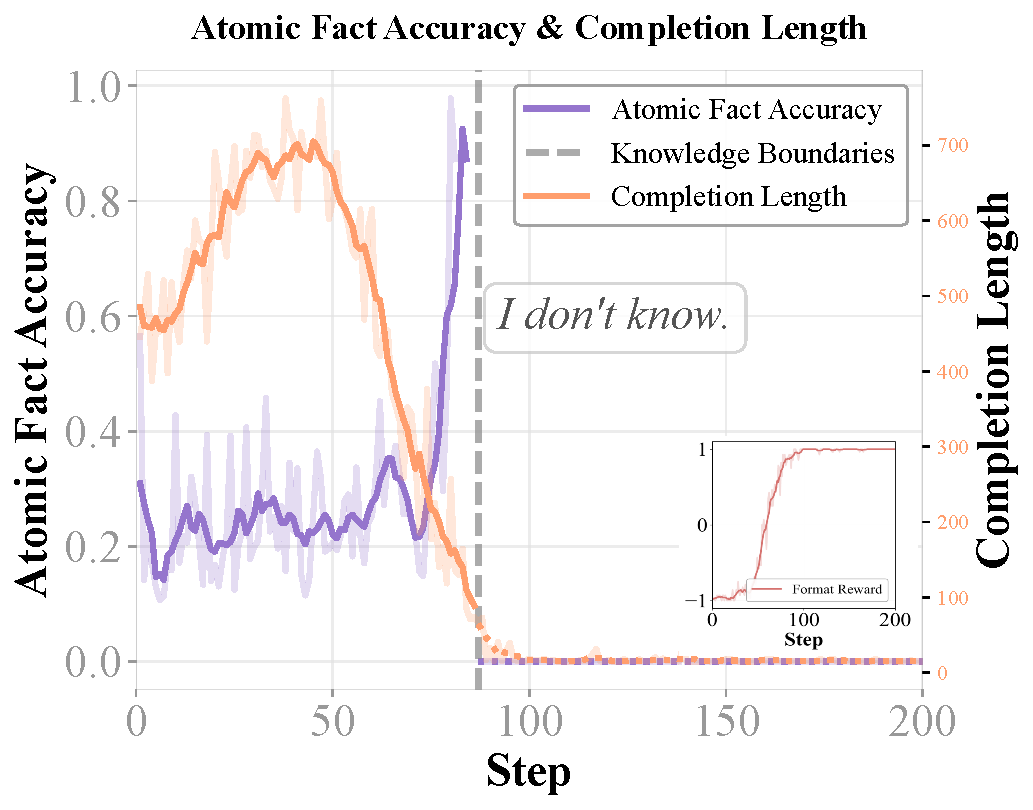
\includegraphics[width=\linewidth]{images/Skywork_final.pdf}
        \caption{The Training Curves (Skywork-OR1-7B-Preview)}
        \label{fig:sub1}
    \end{subfigure}
    \hfill
    \begin{subfigure}[b]{0.32\textwidth}
        \centering
        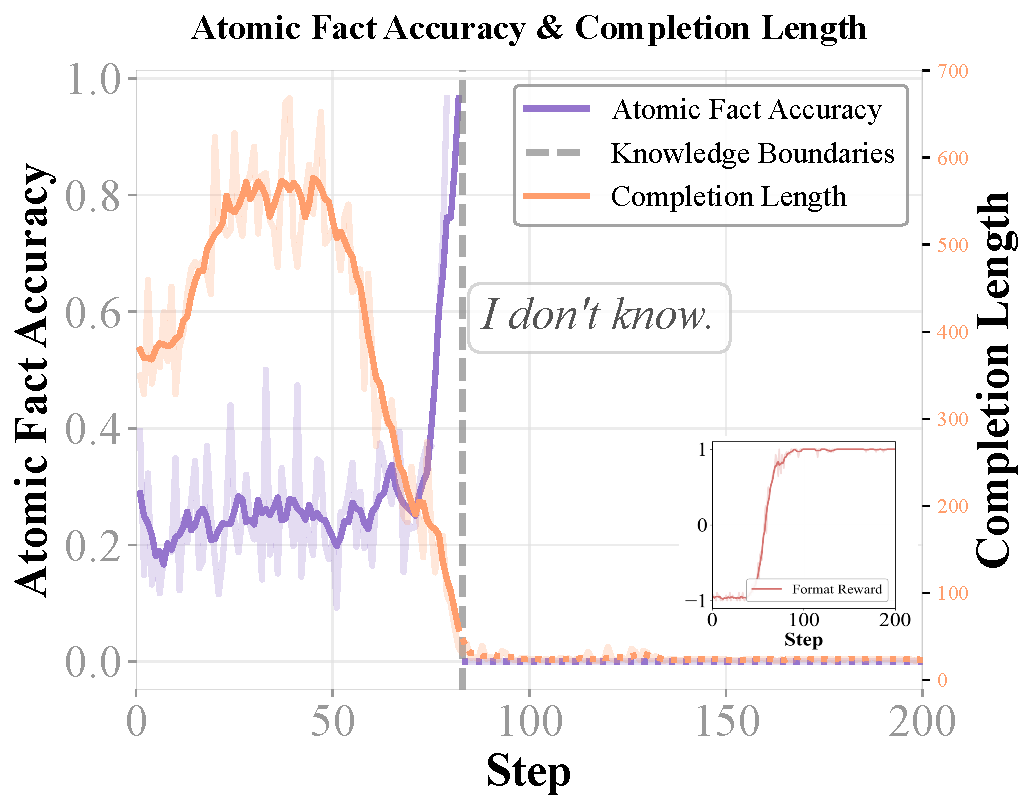
\includegraphics[width=\linewidth]{images/DeepSeek_final.pdf}
        \caption{The Training Curves (DeepSeek-R1-Distill-Qwen-7B)}
        \label{fig:sub2}
    \end{subfigure}
    \hfill
    \begin{subfigure}[b]{0.32\textwidth}
        \centering
        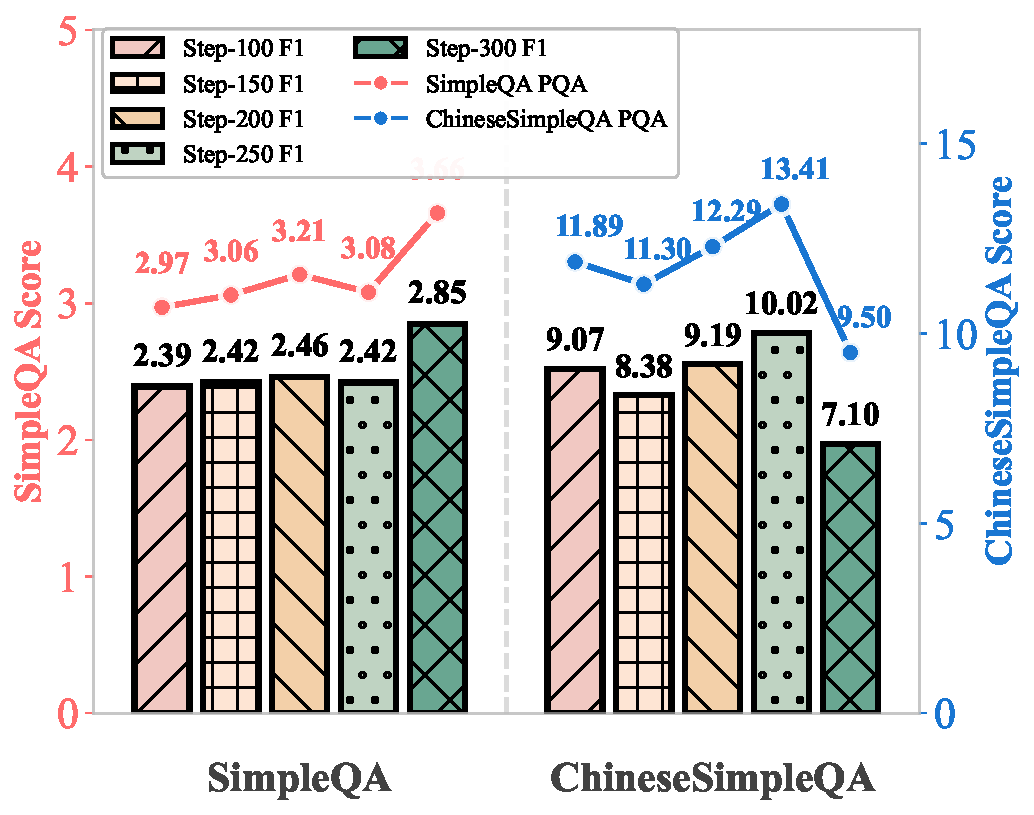
\includegraphics[width=\linewidth]{images/f1_pqa_dual_axis_analysis.pdf}
        \caption{F1 and PAQ Across Training Steps on SimpleQA and ChineseSimpleQA}
        \label{fig:sub3}
    \end{subfigure}
    \hfill
    \begin{subfigure}[b]{0.32\textwidth}
        \centering
        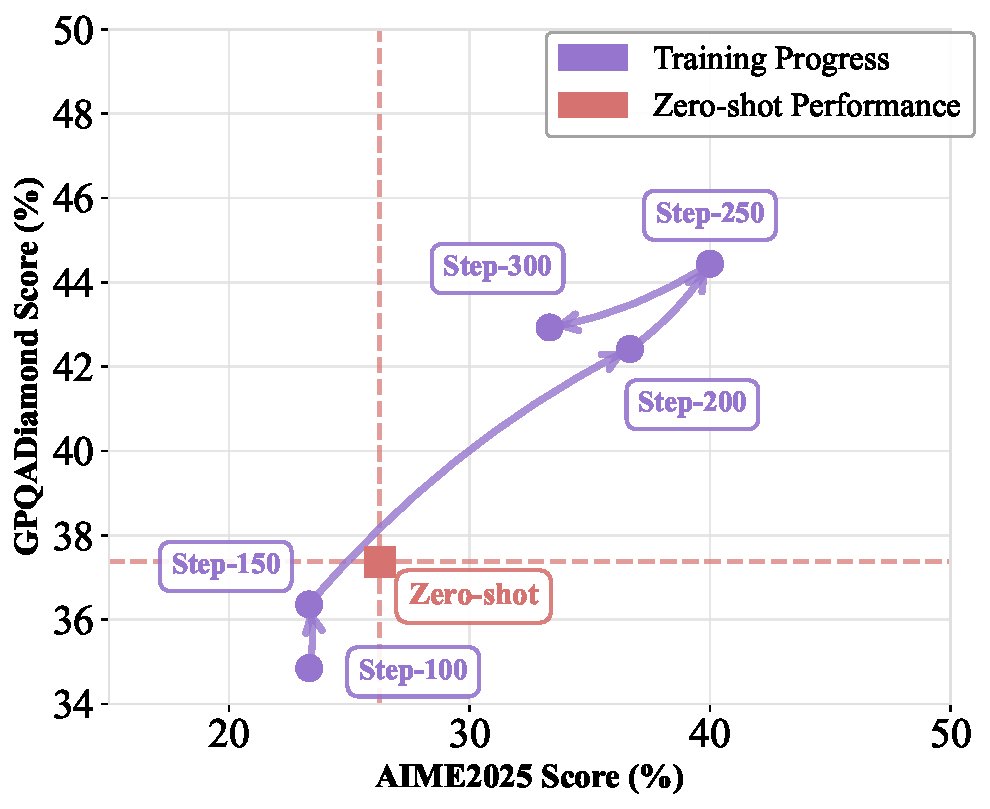
\includegraphics[width=\linewidth]{images/gpqa_aime_analysis.pdf}
        \caption{Training Progress on GPQA and AIME~2025}
        \label{fig:sub4}
    \end{subfigure}
    \hfill
    \begin{subfigure}[b]{0.32\textwidth}
        \centering
        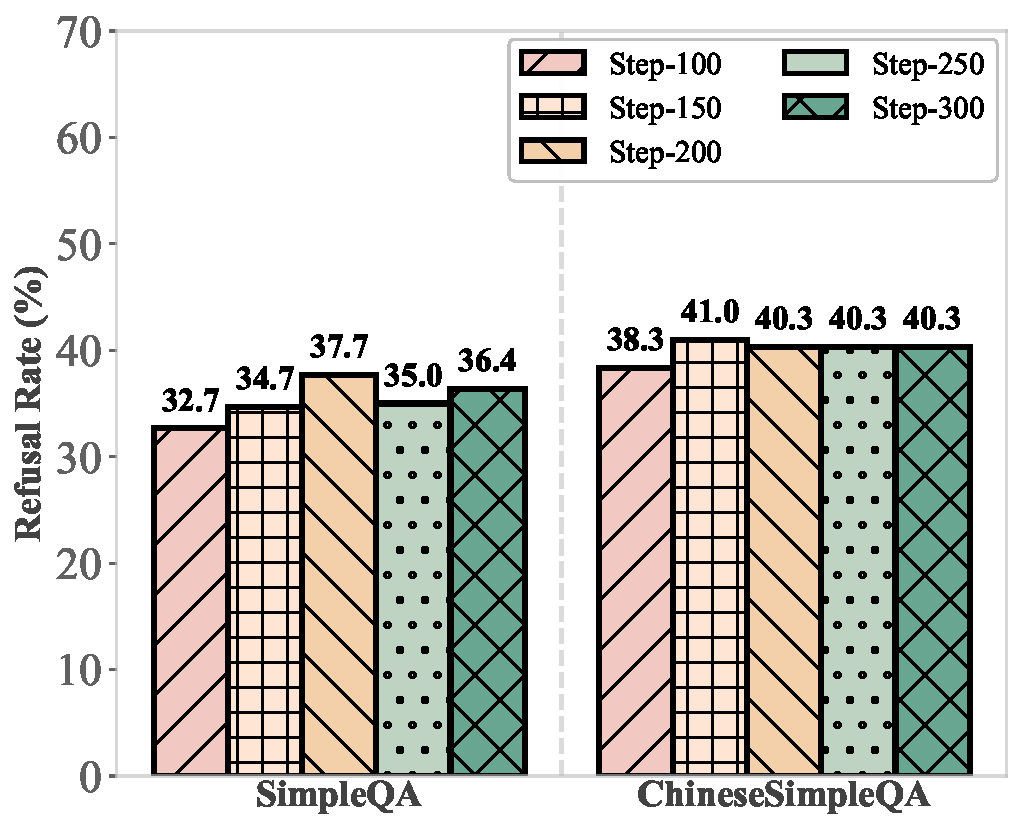
\includegraphics[width=\linewidth]{images/refusal_rates_analysis.pdf}
        \caption{Refusal Rates Across Training Steps on SimpleQA and ChineseSimpleQA}
        \label{fig:sub5}
    \end{subfigure}
    \hfill
    \begin{subfigure}[b]{0.32\textwidth}
        \centering
        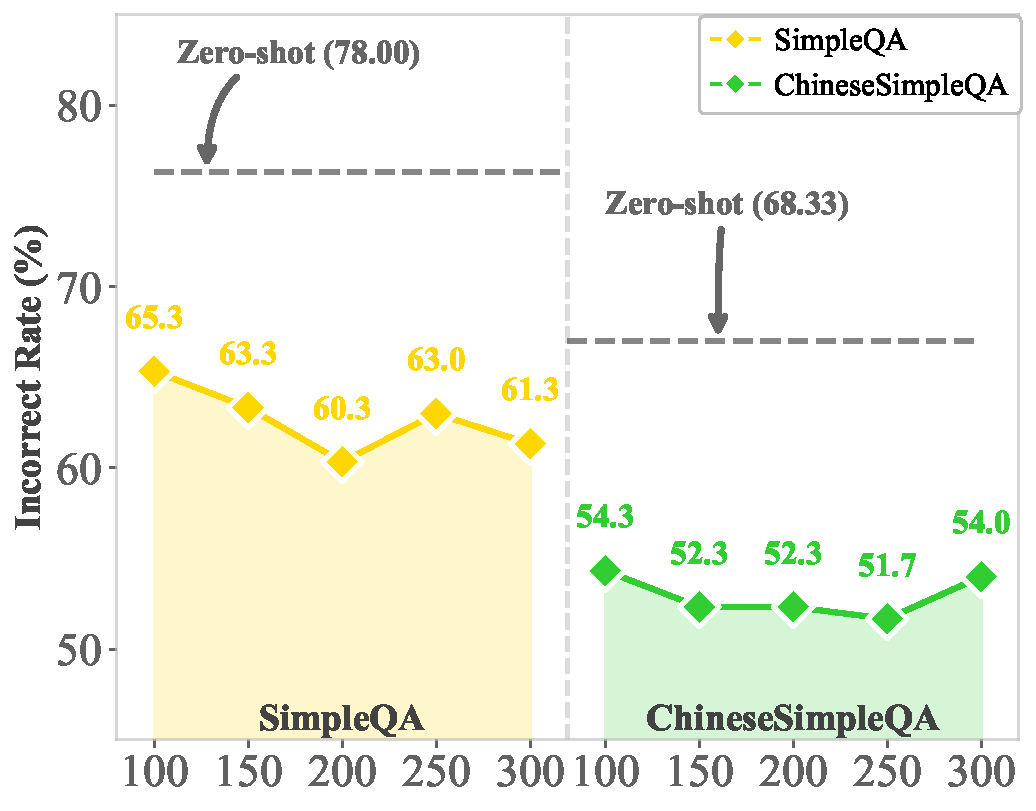
\includegraphics[width=\linewidth]{images/incorrect_rates_baseline_analysis.pdf}
        \caption{Incorrect Rates Across Training Steps vs. Zero-shot Performance}
        \label{fig:sub6}
    \end{subfigure}
    \caption{
    KnowRL training dynamics and reasoning behavior analysis. 
    (a)--(b) present the training curves of two model architectures, showing improved factual alignment and stable reasoning length. 
    (c)--(f) illustrate performance trends of Skywork-OR1-7B-Preview across different training steps, including F1 and PAQ (c), reasoning accuracy (d), refusal rate (e), and incorrect rate (f).
    }
    \vspace{-3ex}
    \label{fig:knowrl-exp}
\end{figure*}



% \begin{table*}[t]
%     \centering
%     \small
%     \setlength{\tabcolsep}{3.2pt}
%     \renewcommand{\arraystretch}{1.2} % Slightly increase row height for readability
%     \begin{tabular}{l|ccc|cc}
%     \toprule
%     \multirow{2}{*}{\makecell[c]{\normalsize\textbf{Reward}}} & \multicolumn{3}{c|}{\textbf{Hallucination}} & \multicolumn{2}{c}{\textbf{Reasoning}} \\
%     \cmidrule(lr){2-4} \cmidrule(lr){5-6}
%     & \small\textbf{TruthfulQA} & \small\textbf{SimpleQA} & \small\textbf{ChineseSimpleQA}  & 
%     \small\textbf{GPQA Diamond} & \small\textbf{AIME 2025}\\
   
%     \midrule
%     \multicolumn{6}{c}{\textbf{DeepSeek-R1-Distill-Qwen-7B}} \\
%     \text{Direct Generation}   & 33.05 & 1.92 & \textbf{11.17}  & 34.34 & 16.67  \\
%     \text{Format}              & 33.41 & \textbf{2.36} & 10.47  & 35.86 & 10.00  \\
%     \text{Format+Fact}         & 34.03 & 1.55 & 9.70  & 31.31 & 16.67  \\
%     \text{Format+Correct}      & \textbf{34.76}  & 1.74 & 10.97 & \textbf{37.88} & \textbf{20.00}  \\
%     \rowcolor{tablehighlight} % Changed color here
%     \text{Format+Fact+Correct} & 33.54 & 1.34 & 11.00 & 34.34 & 6.67  \\
       
%     \midrule
%     \multicolumn{6}{c}{\textbf{DeepSeek-R1-Distill-Qwen-7B-ColdStart}} \\
%     \text{Direct Generation}      & 35.86 & 3.75 & 12.70 & \textbf{39.39} & \textbf{20.00 }  \\
%     \text{Format}                & 36.84 & 3.73 & 14.37 & 35.86 & 16.67  \\
%     \text{Format+Fact}           & 37.82 & \textbf{6.16} & \textbf{14.60} & 35.86 & 13.33 \\
%     \text{Format+Correct}        & 37.82 & 4.04 & 13.80 & 33.33 & 16.67 \\
%     \rowcolor{tablehighlight} % Changed color here
%     \text{Format+Fact+Correct}   & \textbf{38.19} & 4.56 & 13.90 & 37.37 & 13.33 \\
    

%     \bottomrule
%     \end{tabular}
%     \vspace{-1ex}
%     \caption{\textbf{Reward Ablation Experiment.} DeepSeek-R1-Distill-Qwen-7B is trained with cold start to obtain DeepSeek-R1-Distill-Qwen-7B-ColdStart. The best results are marked in \textbf{bold}.}
%     \vspace{-3ex}
%     \label{ablation}
% \end{table*}





\section{Experiments}
\subsection{Experimental Settings.}
\paragraph{Datasets and Metrics.}
We use TruthfulQA~\citep{lin2021truthfulqa}, SimpleQA, and ChineseSimpleQA to evaluate hallucination, and GPQA (general domain) and AIME 2025 (mathematical reasoning) to evaluate reasoning ability.
For the hallucination evaluation datasets, we randomly sample 300 examples from each of TruthfulQA, SimpleQA, and ChineseSimpleQA as test sets.
Because slow-thinking models generate thousands of tokens per query, evaluating full datasets is computationally prohibitive.
A 300-example subset remains highly challenging and provides a statistically valid evaluation, which is a standard practice for long-reasoning tasks.
TruthfulQA is assessed with the ROUGE and BLEU metrics.
For SimpleQA and ChineseSimpleQA, we evaluate performance using four metrics: (1) Incorrect Rate, (2) Refusal Rate, (3) Precision on Answered Questions (PAQ), and (4) $F_1$ score.
PAQ measures the proportion of correctly answered questions among those that the model chooses to answer.
For AIME 2025 and GPQA, we assess reasoning performance based on accuracy metric.
All models are evaluated with the temperature set to 0.


\paragraph{Models and Baselines.}
We select the Skywork-OR1-7B-Preview \citep{skywork-or1-2025} and the DeepSeek-R1-Distill-Qwen-7B for experiments. 
These models represent the two most popular slow thinking training methods: RL, represented by the Skywork-OR1-7B-Preview model, and distillation, represented by the DeepSeek-R1-Distill-Qwen-7B model. 
We select Self-Refine \citep{madaan2023self} as the baseline for prompt engineering, and SFT, DPO, FactTune-FS \citep{tian2023fine} and TruthRL \citep{wei2025truthrl} as the baselines for post-training methods. 
For DPO, we use the distilled DeepSeek-R1 data as the chosen data; for FactTune-FS, the chosen data is composed of the original model's outputs, which are filtered for high factuality using FactScore. 
We use Low-Rank Adaptation \citep[LoRA;][]{hu2022lora} to train all models. Further training details are provided in the Appendix~\ref{appendix:train-set}.

% \paragraph{Training Details.}
% We use Low-Rank Adaptation \citep[LoRA;][]{hu2022lora} to train all models. 
% % For the ColdStart training stage, we train for 4 epochs, with the learning rate set to 1.0e-4 and a batch size of 2. 
% For the reinforcement learning training stage, we train for 200 steps, with the learning rate set to 1.0e-5.  
% More details can be seen in the Appendix. 
% Additionally, we test our method on two new models with distinct architectures, as detailed in the Appendix.


\subsection{Main Results}
\paragraph{KnowRL significantly mitigates hallucination while maintaining reasoning capabilities.}
As shown in Table~\ref{main-exp}, KnowRL consistently improves factual reliability across all datasets. 
For the DeepSeek-R1-Distill-Qwen-7B model, the Incorrect Rate on SimpleQA drops by over 20\% (from 78.00\% to 57.67\%), with similar improvements observed on ChineseSimpleQA. 
Notably, since our training knowledge source is primarily English-based, the consistent gains on ChineseSimpleQA highlight strong cross-lingual transferability, suggesting that KnowRL helps the model internalize a language-agnostic verification behavior rather than merely memorizing language-specific factual patterns.
Importantly, unlike baseline methods that often suffer from catastrophic forgetting, KnowRL preserves strong performance on complex reasoning benchmarks. 
For instance, it improves the GPQA score from 37.37\% to 42.42\% and maintains stability on AIME 2025, demonstrating that factual supervision does not conflict with deep reasoning abilities.
This favorable trade-off can be attributed to KnowRL's process-level design: by rewarding the factual grounding of individual reasoning steps rather than solely adjusting outcome distributions, the model retains its capacity for extended logical deduction while learning to ground each step in verifiable knowledge.
Furthermore, the dramatic drop in completion length (Figure~\ref{fig:knowrl-exp}(a) and (b)) reflects acquired boundary-awareness rather than a collapse of the slow-thinking process.
The model efficiently truncates wasteful hallucinations for unknown facts while preserving extended reasoning chains for complex logical tasks.




\paragraph{Training dynamics demonstrate that the model progressively learns to recognize knowledge boundaries.}
Figure~\ref{fig:knowrl-exp}(a) and (b) illustrates how KnowRL shapes the model's behavior. 
During training, the accuracy of atomic facts within the chain-of-thought steadily increases. 
As the model becomes more precise in its reasoning steps, it learns to distinguish known facts from unknown information. 
Consequently, instead of fabricating answers when uncertain, the model learns to abstain, reflected by a rise in the Refusal Rate and a sharp drop in the Incorrect Rate. 
This confirms that KnowRL effectively teaches the model to reason faithfully rather than merely optimizing for lucky guesses.

% As shown in Table~\ref{main-exp}, KnowRL substantially reduces hallucinations across models and languages. 
% Figure~\ref{fig:knowrl-exp}(a) and (b) further reveal the underlying mechanism. 
% During training, the atomic fact accuracy within the chain-of-thought steadily increases, indicating that the model's reasoning process becomes more grounded in verifiable facts. 
% As factual accuracy improves, the model begins to identify when its knowledge is insufficient and learns to abstain from uncertain statements (e.g., outputting ``I don't know'') rather than fabricating answers. 
% This behavioral change aligns with the quantitative trends in Table~\ref{main-exp}, where a higher atomic fact accuracy corresponds to a lower Incorrect Rate and a higher Refusal Rate.

% Together, these results show that KnowRL instills a fact-grounded reasoning paradigm: the model improves atomic fact correctness, becomes aware of its knowledge boundaries, and substantially reduces hallucinations without compromising reasoning ability on datasets such as GPQA and AIME~2025.






% \paragraph{Distillation-based slow-thinking models exhibit a higher training ceiling compared to slow-thinking models trained by RL.} 
% The training curves in Figure~\ref{knowrl-exp} show DeepSeek-R1-Distill-Qwen-7B model achieving a higher combined reward during KnowRL training, with its output length decreases around 110 steps. 
% In contrast, Skywork-OR1-7B-Preview's reward curve during KnowRL training converges to only approximately -0.4. 
% This indicates better training performance for distillation-based models like DeepSeek-R1-Distill-Qwen-7B. 
% This is further supported by Table~\ref{main-exp}, where the KnowRL-trained DeepSeek-R1-Distill-Qwen-7B outperforms all baselines on three hallucination evaluation datasets, while the KnowRL-trained Skywork-OR1-7B-Preview only exceeds all baselines on the ChineseSimpleQA dataset.

% KnowRL's training effect is less pronounced on the initially RL-trained Skywork-OR1-7B-Preview model compared to the distilled DeepSeek-R1-Distill-Qwen-7B. 
% This suggests that RL-trained models might approach a capability ceiling due to converging to a local optimum during their initial RL process, making further improvement by KnowRL difficult due to search space constraints.
% The findings from Reinforcement Learning with Verifiable Rewards \citep[RLVR;][]{yue2025does} support the conclusion that distilled models possess a higher performance ceiling. 
% This is because, unlike methods that merely improve sampling efficiency by narrowing the reasoning search space, distillation allows models to learn genuinely new knowledge from an unreduced search space, enabling more significant enhancement via subsequent RL. 
% Thus, our method effectively reduces hallucination in distilled models, demonstrating its practical utility, and also confirms that stacked RL training can help mitigate hallucinations.

% \begin{table*}[h]
%     \centering
%     \footnotesize 
%     \setlength{\tabcolsep}{3.0pt} 
%     % --- Using @{...} to add extra space after the 'Incorr.' columns ---
%     \begin{tabular}{l|cc@{\hskip 14pt}cc|cc@{\hskip 14pt}cc|cc}
%     \toprule
%     \multirow{3}{*}{\makecell[c]{\textbf{Reward}\\\textbf{Combination}}} & \multicolumn{8}{c|}{\textbf{Hallucination}} & \multicolumn{2}{c}{\textbf{Reasoning}} \\
%     \cmidrule(lr){2-9} \cmidrule(lr){10-11}
%     & \multicolumn{4}{c|}{\textbf{SimpleQA}} & \multicolumn{4}{c|}{\textbf{ChineseSimpleQA}} & \multirow{2}{*}{\makecell[c]{\small\textbf{GPQA}\\\small\textbf{Diamond}}} & \multirow{2}{*}{\small\textbf{AIME}}\\
%     \cmidrule(lr){2-5} \cmidrule(lr){6-9}
%     & \small\textbf{PAQ} & \small\textbf{Incorrect} & \small\textbf{Refusal} & \small\textbf{F1} & \small\textbf{PAQ} & \small\textbf{Incorrect} & \small\textbf{Refusal} & \small\textbf{F1} & & \\
    
%     \midrule
%     \rowcolor{lightgray} \multicolumn{11}{c}{\textit{\textbf{DeepSeek-R1-Distill-Qwen-7B}}} \\
%     \midrule
%     $R = r_{\text{format}}$ & 2.63 & 74.00 & 24.00 & \underline{2.27} & 7.08 & 74.33 & 20.00 & 6.29 & \underline{39.39} & 30.00  \\
%     $R = r_{\text{format}} + r_{\text{fact}}$ & 2.42 & \perf{80.67}{+6.67} & 17.33 & 2.19 & 8.87 & \perf{75.33}{+1.00} & 17.33 & \underline{8.03} & \textbf{47.47} & \textbf{40.00} \\
%     $R = r_{\text{format}} + r_{\text{correct}}$ & \textbf{3.19} & \perf{60.67}{-13.3} & \underline{37.33} & \textbf{2.46} & \underline{8.89} & \perf{41.00}{-33.3} & \textbf{55.00} & 5.52 & 38.89 & \textbf{40.00} \\
%     $R = R_{total}$ (\textbf{KnowRL}) & \underline{2.81} & \perf{57.67}{-16.3} & \textbf{40.67} & 2.09 & \textbf{10.26} & \perf{58.33}{-16.0} & \underline{35.00} & \textbf{8.08} & 37.37 & \underline{33.33} \\
%     \addlinespace[0.5pt] % Adjust the space here
%     KnowRL ($R_{refusal}=-1$) & 1.26 & \perf{78.67}{+4.67} & 20.33 & 1.11 & 7.66 & \perf{84.33}{+10.0} & 8.67 & 7.32 & 34.85 & 30.00 \\
    
%     \bottomrule
%     \end{tabular}
%     \caption{\textbf{Ablation Study.} Ablation study on different reward combinations for the DeepSeek-R1-Distill-Qwen-7B model. The best results are marked in \textbf{bold}, and the second-best results are \underline{underlined}.}
%     \vspace{-3ex}
%     \label{tab:ablation}
% \end{table*}

%$R_{correct}(o=refusal)=-1$




\begin{table*}[h]
    \centering
    \footnotesize 
    \setlength{\tabcolsep}{3.0pt} 
    % --- Using @{...} to add extra space after the 'Incorr.' columns ---
    \begin{tabular}{l|cc@{\hskip 14pt}cc|cc@{\hskip 14pt}cc|cc}
    \toprule
    \multirow{3}{*}{\makecell[c]{\textbf{Method}}} & \multicolumn{8}{c|}{\textbf{Hallucination}} & \multicolumn{2}{c}{\textbf{Reasoning}} \\
    \cmidrule(lr){2-9} \cmidrule(lr){10-11}
    & \multicolumn{4}{c|}{\textbf{SimpleQA}} & \multicolumn{4}{c|}{\textbf{ChineseSimpleQA}} & \multirow{2}{*}{\makecell[c]{\small\textbf{GPQA}\\\small\textbf{Diamond}}} & \multirow{2}{*}{\small\textbf{AIME}}\\
    \cmidrule(lr){2-5} \cmidrule(lr){6-9}
    & \small\textbf{PAQ} & \small\textbf{Incorrect} & \small\textbf{Refusal} & \small\textbf{F1} & \small\textbf{PAQ} & \small\textbf{Incorrect} & \small\textbf{Refusal} & \small\textbf{F1} & & \\
    
    \midrule
    \rowcolor{lightgray} \multicolumn{11}{c}{\textit{\textbf{Ablation on Reward Combination (Base Model: DeepSeek-R1-Distill-Qwen-7B)}}} \\
    \midrule
    $R = r_{\text{format}}$ & 2.63 & 74.00 & 24.00 & \underline{2.27} & 7.08 & 74.33 & 20.00 & 6.29 & \underline{39.39} & 30.00  \\
    $R = r_{\text{format}} + r_{\text{fact}}$ & 2.42 & \perf{80.67}{+6.67} & 17.33 & 2.19 & 8.87 & \perf{75.33}{+1.00} & 17.33 & \underline{8.03} & \textbf{47.47} & \textbf{40.00} \\
    $R = r_{\text{format}} + r_{\text{correct}}$ & \textbf{3.19} & \perf{60.67}{-13.33} & \underline{37.33} & \textbf{2.46} & \underline{8.89} & \perf{41.00}{-33.33} & \textbf{55.00} & 5.52 & 38.89 & \textbf{40.00} \\
    $R = R_{total}$ (KnowRL) & \underline{2.81} & \perf{57.67}{-16.33} & \textbf{40.67} & 2.09 & \textbf{10.26} & \perf{58.33}{-16.00} & \underline{35.00} & \textbf{8.08} & 36.87 & \underline{33.33} \\
    \addlinespace[0.5pt] % Adjust the space here
    KnowRL ($R_{refusal}=-1$) & 1.26 & \perf{78.67}{+4.67} & 20.33 & 1.11 & 7.66 & \perf{84.33}{+10.00} & 8.67 & 7.32 & 34.85 & 30.00 \\
    
    \addlinespace[2pt]
    \midrule
    \rowcolor{lightgray} \multicolumn{11}{c}{\textit{\textbf{Robustness Analysis (Using GRPO reward, $R = R_{total}$)}}}\\
    \midrule
    
    Zero-shot & 2.09 & 78.00 & 20.33 & 1.86 & 8.07 & 68.33 & 25.67 & 6.88 & 40.91 & 30.00 \\
    \addlinespace[0.5pt]
    KnowRL (DAPO) & 1.11 & \perf{59.33}{-18.67} & 40.00 & 0.83 & 9.14 & \perf{59.67}{-8.66} & 34.33 & 7.24 & 41.41 & 43.33 \\
    KnowRL (BNPO) & 1.61 & \perf{61.00}{-17.00} & 38.00 & 1.23 & 11.48 & \perf{61.67}{-6.66} & 30.33 & 9.43 & 41.41 & 30.00 \\
    KnowRL (Dr.GRPO) & 3.16 & \perf{61.33}{-16.67} & 36.67 & 2.45 & 11.33 & \perf{60.00}{-8.33} & 32.33 & 9.15 & 38.38 & 43.33 \\

    \bottomrule
    \end{tabular}
    \caption{\textbf{Ablation and Robustness Analysis.} Impact of reward components and different RL algorithms for the DeepSeek-R1-Distill-Qwen-7B. In reward ablation section, best results are in \textbf{bold} and second-best are \underline{underlined}.}
    \vspace{-3ex}
    \label{tab:ablation}
\end{table*}





















\subsection{Extended Evaluation on Reasoning Benchmarks}
We further evaluate KnowRL on OlympiadBench~\citep{he2024olympiadbench} to examine its impact on complex reasoning in mathematics and physics. 
As shown in Table~\ref{tab:olympiadbench_optimized_concise}, both models maintain or improve their performance after KnowRL training. 
Specifically, the DeepSeek model increases its average accuracy from 7.23\% to 7.58\%, while the Skywork model improves from 4.65\% to 5.75\%. 
Both models achieved significant gains in the Chinese physics task (\textit{physics\_zh\_CEE}), with DeepSeek-7B rising from 7.83\% to 11.30\%. 
Although there are minor fluctuations in individual sub-tasks, the overall trend confirms that factual supervision does not hinder structured reasoning.


Combined with the consistent results on GPQA and AIME~2025, these findings provide strong evidence that \textbf{KnowRL effectively preserves and enhances complex reasoning capabilities across diverse other domains, enabling models to reason more reliably under factual constraints}.





\subsection{Training Step Analysis}
To investigate how the number of KnowRL training steps affects the trade-off between factuality and reasoning, we evaluate models trained for 100, 150, 200, 250, and 300 reinforcement learning steps. 
The results are illustrated in Figure~\ref{fig:knowrl-exp}(c)--(f).

As shown in Figure~\ref{fig:knowrl-exp}(c), both F1 and PAQ scores improve rapidly in the early stage of training and reach a stable high level after moderate training, suggesting that factual precision and reliability are primarily acquired in the middle phase of optimization. 
Reasoning performance on GPQA and AIME~2025 (Figure~\ref{fig:knowrl-exp}(d)) remains stable or slightly improves within this range, indicating that factual supervision can refine reasoning without inducing degradation. 
Refusal rates (Figure~\ref{fig:knowrl-exp}(e)) increase and then plateau, reflecting that models progressively learn appropriate abstention behavior, while the incorrect rate (Figure~\ref{fig:knowrl-exp}(f)) decreases sharply in early training and stabilizes thereafter. 
Beyond this stage, additional optimization provides limited factual improvement and introduces minor task-dependent variations rather than consistent gains.

These observations suggest that KnowRL’s reinforcement learning dynamics follow a stable convergence pattern rather than the reversal effects sometimes observed in overfitted reasoning models~\citep{berglund2023reversal}. 
Appropriate training duration is therefore crucial: insufficient updates hinder factual learning, whereas excessive optimization may overfit factual supervision signals and weaken generalization.

\textbf{Overall, KnowRL achieves its best balance between factuality and reasoning stability when trained for an appropriate number of reinforcement learning steps, where the model fully internalizes factual supervision without over-optimization or reasoning drift.}


\subsection{Ablation Study}

%\subsection{Impact of Reward Components}

To understand how different reward signals contribute to the model's performance, we evaluate the DeepSeek-R1-Distill-Qwen-7B model under different reward combinations.

\paragraph{Factual reward ($r_{fact}$) enhances fact-grounded reasoning.}
As shown in Table~\ref{tab:ablation}, using the factual reward alone achieves the best performance on reasoning benchmarks such as GPQA and AIME~2025. 
This shows that $r_{\text{fact}}$ encourages models to perform reasoning grounded in verifiable knowledge, helping them maintain accuracy while reducing random errors. 
This finding underscores the importance of factual verification in the reinforcement learning process, consistent with prior work showing that incorporating verifiable rewards can substantially improve the reliability and stability of RL training~\citep[RLVR;][]{yue2025does}.


\paragraph{Positive refusal incentives promote boundary awareness.} Table~\ref{tab:ablation} shows that giving a positive reward for refusals leads to higher refusal rates and fewer hallucination errors. 
This explicitly encourages the model to admit when it lacks knowledge.
When we removed this positive incentive (setting $R_{\text{refusal}}=-1$), the incorrect rate increased significantly.
This confirms that rewarding appropriate refusals is essential for learning knowledge boundaries.

% \paragraph{Correct reward ($r_{\text{correct}}$) with positive refusal incentives promotes boundary awareness.}
% Table~\ref{tab:ablation} shows that the positive reward assigned to refusals in $r_{\text{correct}}$ leads to higher refusal rates and lower hallucination errors, indicating that such design explicitly encourages the model to recognize when it lacks sufficient knowledge and to abstain from unreliable responses. 
% To further verify that the refusal reward is the key factor driving boundary awareness, we set $R_{\text{correct}}(o \in \text{refusal}) = -1$ in KnowRL and obtain the results of KnowRL ($R_{\text{refusal}}=-1$). 
% As shown in Table~\ref{tab:ablation}, the incorrect rate rises substantially under this setting, confirming that rewarding appropriate refusals is essential for stimulating boundary learning and mitigating hallucinations. 
% This finding aligns with recent analyses of reward shaping for truthful generation~\citep{shao2025spurious}, which emphasize that correctly incentivizing uncertainty recognition is critical for enhancing factual reliability in reinforcement learning–based language models.



% \paragraph{Simple reward combinations are insufficient for mitigating hallucination in factual tasks.} 
% As demonstrated in Table~\ref{ablation}, using simple reward combinations, for example 'Format' and 'Correct' rewards, can even decrease the performance of the DeepSeek-R1-Distill-Qwen-7B on the SimpleQA dataset. 
% This suggests that for open-domain factual tasks, a model can learn to generate answers that satisfy the correctness reward without adhering to a factual reasoning process. Our finding presents a notable contrast to observations in other domains like mathematical reasoning. There, some research suggests that simpler reward combinations can yield performance gains, even if by capitalizing on spurious signals \citep{shao2025spurious}. 
% We, therefore, conclude that for the complex challenge of mitigating hallucinations, a simple combination of rewards is not a reliable solution, underscoring the need for a more comprehensive approach like the full KnowRL framework.

\section{Analysis}

\subsection{Robustness Analysis of Different RL Algorithms}

To verify that the effectiveness of KnowRL is not limited to a specific optimization method, we extended our framework to three additional RL algorithms: BNPO \cite{xiao2025bnpo}, DAPO \citep{yu2025dapo}, and Dr.GRPO \citep{liu2025understanding}. 
We compare their performance using the DeepSeek-R1-Distill-Qwen-7B model.

\paragraph{KnowRL is robust across different algorithms.} 
Table~\ref{tab:ablation} demonstrates that every algorithm achieved the dual goal of our framework: they all significantly reduced the Incorrect Rate compared to the Zero-shot baseline, while successfully maintaining or even improving reasoning performance. 
This confirms that the KnowRL framework effectively reduces hallucinations without compromising reasoning capabilities, regardless of the specific RL algorithm used. 
Detailed analysis of response length and atomic fact accuracy during training is provided in Appendix~\ref{appendix:RL_algorithms}.







\subsection{Analysis of Factors Affecting Knowledge Boundaries}

To examine whether the positive refusal reward in $r_{\text{correct}}$ is the only factor driving boundary learning, we conducted an experiment on the DeepSeek-R1-Distill-Qwen-7B model using SimpleQA and ChineseSimpleQA. 
We modified the KnowRL setting by changing the refusal reward from positive to negative $r_{\text{refusal}=-1}$, while keeping other rewards unchanged. 
We evaluated the model at training steps 0, 100, 150, 200, and 250.

As shown in Figure~\ref{fig:boundary-analysis}, the refusal rate initially rises even without a positive refusal reward. 

This confirms that the positive refusal reward is not the only factor affecting knowledge boundaries; the penalty for incorrect answers also encourages the model to be cautious in the early stages. 
However, this behavior is unstable. 
Later stages in Figure~\ref{fig:boundary-analysis} show a significant drop in refusal rates accompanied by a spike in incorrect answers. 
This occurs because the model learns to guess to maximize scores rather than accepting refusal penalties—known as reward hacking. Thus, while correctness rewards trigger initial caution, positive refusal rewards are essential to maintain it and prevent guessing.
\textbf{Overall, the results suggest that positive refusal rewards are not the only source of boundary learning; 
different reward combinations can jointly promote boundary-aware reasoning.}



We further investigate the scalability and evaluator sensitivity of our framework. 
Experiments on the larger DeepSeek-R1-Distill-Qwen-14B model show that KnowRL consistently reduces hallucinations while improving reasoning capabilities, confirming its scalability across model sizes(details in Appendix~\ref{appendix:scalability}). 
Moreover, we conduct an Evaluator Sensitivity Analysis by replacing the GPT-4o-mini used during training with different model. 
The results indicate that KnowRL maintains robust performance regardless of the specific evaluator used. Comprehensive results for these analyses are provided in Appendix~\ref{appendix:sensitivity}.


\begin{figure}[t]
    \centering
    \resizebox{.41\textwidth}{!}{
    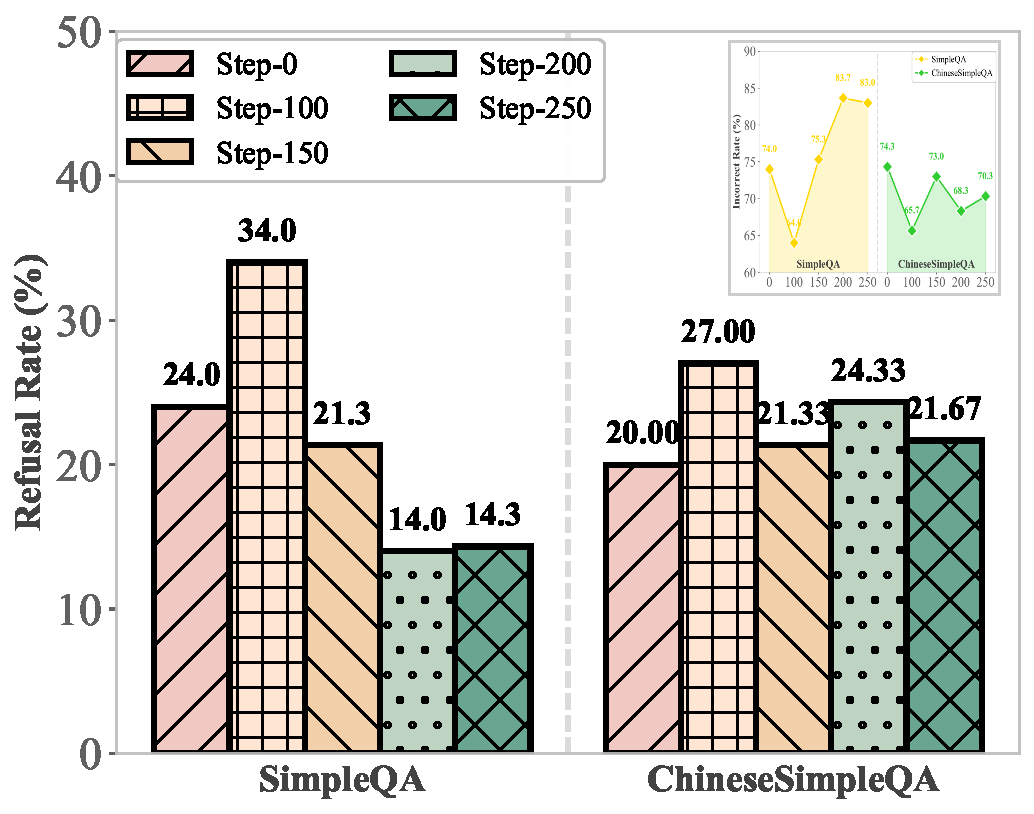
\includegraphics{images/refusal_rates_analysis_with_inset.pdf}}
    \caption{
    Trends of refusal and incorrect rates on SimpleQA and ChineseSimpleQA 
    when training with the combination of format reward and negative refusal reward across different training steps.}
    \vspace{-3ex}
    \label{fig:boundary-analysis}
\end{figure}






\section{Robustness and Multi-run Evaluation}
\label{app:multi_run}

To address the potential sensitivity of single-run evaluations at zero temperature, especially on small-scale benchmarks like AIME, we conduct a robust multi-run evaluation.
We re-evaluate the base models and KnowRL using a non-zero temperature of 0.6, generating 5 responses per prompt to report the average performance (Avg@5).
This setup ensures that the observed improvements in factuality and reasoning are consistent and not artifacts of decoding variance.

\begin{table*}[t]
    \centering
    \footnotesize 
    \setlength{\tabcolsep}{3.0pt} 
    \begin{tabular}{l|cc|cc@{\hskip 10pt}cc|cc@{\hskip 10pt}cc|cc}
    \toprule
    \multirow{3}{*}{\makecell[c]{\textbf{Methods}}} & \multicolumn{10}{c|}{\textbf{Hallucination}} & \multicolumn{2}{c}{\textbf{Reasoning}} \\
    \cmidrule(lr){2-11} \cmidrule(lr){12-13}
    & \multicolumn{2}{c|}{\textbf{TruthfulQA}} & \multicolumn{4}{c|}{\textbf{SimpleQA}} & \multicolumn{4}{c|}{\textbf{ChineseSimpleQA}} & \multirow{2}{*}{\makecell[c]{\small\textbf{GPQA}\\\small\textbf{Diamond}}} & \multirow{2}{*}{\small\textbf{AIME}}\\
    \cmidrule(lr){2-3} \cmidrule(lr){4-7} \cmidrule(lr){8-11}
    & \small\textbf{Rouge} & \small\textbf{Bleu} & \small\textbf{PAQ} & \small\textbf{Incorrect} & \small\textbf{Refusal} & \small\textbf{F1} & \small\textbf{PAQ} & \small\textbf{Incorrect} & \small\textbf{Refusal} & \small\textbf{F1} & & \\
    \midrule
    \rowcolor{lightgray} \multicolumn{13}{c}{\textit{\textbf{Skywork-OR1-7B-Preview}}} \\
    \midrule
    \text{Zero-shot}    & 56.20 & 51.60 & 7.48 & 59.47 & 35.73 & 9.16 & 10.95 & 57.87 & 35.00 & 13.30 & 44.95 & 34.67  \\
    \text{DPO}          & 56.13 & 51.33 & 6.65 & \perf{81.27}{+21.80} & 12.93 & 10.93 & 11.83 & \perf{77.47}{+19.60} & 12.13 & 18.81 & 44.34 & 34.67 \\
    \text{FactTune-FS}  & 57.60 & 53.00 & 3.51 & \perf{44.33}{-15.14} & 54.07 & 2.20 & 10.84 & \perf{40.60}{-17.27} & 54.47 & 9.40 & 45.45 & 34.67  \\
    \text{SFT}          & 57.27 & 50.93 & 9.52 & \perf{61.07}{+1.60} & 32.40 & 10.71 & 8.21 & \perf{78.93}{+21.06} & 14.00 & 7.59 & 39.39 & 38.67  \\
    \text{TruthRL}      & 57.67 & 53.47 & 8.15 & \perf{49.07}{-10.40} & 46.60 & 8.30 & 12.33 & \perf{32.60}{-25.27} & 62.80 & 8.78 & 46.36 & 33.33 \\
    \text{KnowRL}       & 58.27 & 52.80 & 7.32 & \perf{40.20}{-19.27} & \textbf{56.60} & 6.17 & 10.30 & \perf{28.40}{-29.47} & \textbf{68.33} & 6.32 & \textbf{48.89} $\uparrow$ & \textbf{38.00} $\uparrow$ \\[3pt]
    \midrule
    \rowcolor{lightgray} \multicolumn{13}{c}{\textit{\textbf{DeepSeek-R1-Distill-Qwen-7B}}} \\
    \midrule
    \text{Zero-shot}    & 57.40 & 51.53 & 4.89 & 62.47 & 34.33 & 6.20 & 10.23 & 60.27 & 32.93 & 11.83 & 45.45 & 29.33  \\
    \text{DPO}          & 55.60 & 51.40 & 5.65 & \perf{76.33}{+13.86} & 19.07 & 8.74 & 9.54 & \perf{67.20}{+6.93} & 25.73 & 13.20 & 40.40 & 28.67 \\
    \text{FactTune-FS}  & 56.93 & 52.13 & 2.73 & \perf{61.73}{-0.74} & 36.53 & 2.12 & 8.90 & \perf{56.60}{-3.67} & 37.87 & 10.48 & 43.74 & 30.67  \\
    \text{SFT}          & 57.13 & 51.27 & 9.38 & \perf{82.47}{+20.00} & 9.00 & 15.72 & 9.86 & \perf{82.07}{+21.80} & 8.93 & 9.41 & 38.28 & 35.33  \\
    \text{TruthRL}      & 56.27 & 51.94 & 5.93 & \perf{50.73}{-11.74} & 46.07 & 6.19 & 9.37 & \perf{30.47}{-29.80} & 66.40 & 4.69 & 44.34 & 31.33 \\
    \text{KnowRL}       & 57.20 & 52.40 & 5.50 & \perf{48.27}{-14.20} & \textbf{48.93} & 5.43 & 8.38 & \perf{28.07}{-32.20} & \textbf{69.40} & 4.94 & \textbf{46.97} $\uparrow$ & \textbf{34.00} $\uparrow$ \\
    \bottomrule
    \end{tabular}
    \caption{\textbf{Multi-run Evaluation Results.} Robust multi-run performance (Avg@5, Temperature=0.6) of KnowRL compared against baselines on the Skywork-OR1-7B-Preview and DeepSeek-R1-Distill-Qwen-7B models. Zero-shot refers to the original model performance. The key improvements are marked in \textbf{bold}.}
    \vspace{-3ex}
    \label{tab:multi_run_results}
\end{table*}

As shown in Table \ref{tab:multi_run_results}, the multi-run averages consistently support our primary findings.
Even under stochastic decoding, KnowRL significantly improves refusal rates on hallucination-prone queries (SimpleQA and ChineseSimpleQA) while simultaneously enhancing or maintaining performance on complex reasoning tasks (GPQA and AIME).
For instance, KnowRL improves AIME accuracy from 29.33\% to 34.00\% for DeepSeek-7B, confirming that our framework effectively promotes reliable reasoning rather than simply collapsing to conservative refusals.















% \begin{table*}[!htbp]
%     \centering
%     \small
%     \setlength{\tabcolsep}{3.2pt}
%     \renewcommand{\arraystretch}{1.2} % Slightly increase row height for readability
%     \begin{tabular}{l|ccc|cc}
%     \toprule
%     \multirow{2}{*}{\makecell[c]{\normalsize\textbf{KnowRL}}} & \multicolumn{3}{c|}{\textbf{Hallucination}} & \multicolumn{2}{c}{\textbf{Reasoning}} \\
%     \cmidrule(lr){2-4} \cmidrule(lr){5-6}
%     & \small\textbf{TruthfulQA} & \small\textbf{SimpleQA} & \small\textbf{ChineseSimpleQA}  & 
%     \small\textbf{GPQA} & \small\textbf{AIME 2025}\\
   
%     \midrule
%     \multicolumn{6}{c}{\textbf{Skywork-OR1-7B-Preview}} \\
%    \text{Direct Generation}     & 34.39 & 4.58 & 13.27  & 31.31 & 6.67  \\
%    % \text{SFT (ColdStart)}     & 35.99 & 5.14 & 14.67 & 33.84 & 20.00   \\
%     \text{KnowRL Step100}        & 37.45 & 4.31 & 16.37 & 35.86 & 20.00 \\
%     \text{KnowRL Step150}        & 37.70 & 5.04 & 16.23 & 34.34 & 10.00 \\
%     \text{KnowRL Step200}        & 36.96 & 4.82 & 15.33 & 34.34 & 10.00  \\
       
%     % \midrule
%     % \multicolumn{6}{c}{\textbf{DeepSeek-R1-Distill-Qwen-7B}} \\
%     % \text{Direct Generation}     & 33.05 & 1.92 & 11.17  & 34.34 & 16.67  \\
%     % \text{KnowRL Step100}        & 33.17 & 1.25 & 11.17 & 34.34 & 13.33 \\
%     % \text{KnowRL Step150}        & 33.54 & 1.34 & 11.00 & 34.34 & 6.67  \\
%     % \text{KnowRL Step200}        & 35.50 & 2.03 & 9.83 & 33.83 & 6.67   \\

%     % \midrule
%     \multicolumn{6}{c}{\textbf{DeepSeek-R1-Distill-Qwen-7B}} \\
%     %\text{SFT (ColdStart)}       & 35.86 & 3.75 & 12.70 & 38.89 & 20.00   \\
%     \text{Direct Generation}     & 33.05 & 1.92 & 11.17  & 34.34 & 16.67  \\
%     \text{KnowRL Step100}        & 36.60 & 3.76 & 14.47 & 35.86 & 20.00 \\
%     \text{KnowRL Step150}        & 38.19 & 4.79 & 13.90 & 36.36 & 16.67  \\
%     \text{KnowRL Step200}        & 36.72 & 4.46 & 12.83 & 37.37 & 16.67   \\
%     %\text{KnowRL Step250}        & 35.74 & 4.51 & 14.07 & 36.36 & 16.67
%     \end{tabular}
%     \vspace{-1ex}
%     \caption{ Main Experiment}
%     \vspace{-3ex}
%     \label{train-step}
% \end{table*}





% \begin{table*}[t!]
%     \centering
%     \small
%     \setlength{\tabcolsep}{3.2pt}
%     \renewcommand{\arraystretch}{1.2} % Slightly increase row height for readability
%     \begin{tabular}{l|ccc|cc}
%     \toprule
%     \multirow{2}{*}{\makecell[c]{\normalsize\textbf{KnowRL}}} & \multicolumn{3}{c|}{\textbf{Hallucination}} & \multicolumn{2}{c}{\textbf{Reasoning}} \\
%     \cmidrule(lr){2-4} \cmidrule(lr){5-6}
%     & \small\textbf{TruthfulQA} & \small\textbf{SimpleQA} & \small\textbf{ChineseSimpleQA}  & 
%     \small\textbf{GPQA} & \small\textbf{AIME 2025}\\
   
%     \midrule
%     \multicolumn{6}{c}{\textbf{DeepSeek-R1-Distill-Qwen-7B}} \\
%     \text{ColdStart (1.8K) }     & 35.86 & 3.75 & 12.70 & 39.39 & 20.00  \\
%     \text{KnowRL (1.8K) }       & 38.19 & 4.79 & 13.90 & 36.36 & 16.67  \\
%     \text{ColdStart (3K)}        & 36.23 & 3.54 & 12.03 & 34.34 & 16.67 \\
%     \text{KnowRL (3K) }         & 35.25 & 4.26 & 14.13 & 36.36 & 20.00  \\
    
%     \bottomrule
%     \end{tabular}
%     \vspace{-1ex}
%     \caption{Cold start data size analysis.}
%     \vspace{-3ex}
%     \label{coldstart-data}
% \end{table*}








\section{Related Work}
\paragraph{Hallucination Mitigation.} 
% The hallucination in LLMs has attracted significant attention from both academic and industry researchers. 
% Hallucination emerge for a variety of reasons, including noise in the training data, the model's intrinsic creative tendencies, and misjudgment of its own knowledge boundaries \citep{zhang2023user,tonmoy2024comprehensive,liang2024learning}. 
% Existing hallucination mitigation methods are diverse. 
% Prompt engineering approaches, for instance, guide models towards factual content using specific prompts or self-reflection for error correction \citep{sinha2023mathematical,zhang2024self}. 
% Other methods include fine-tuning to enhance facticity on specific tasks \citep{tian2023fine}, Retrieval Augmented Generation (RAG) which utilizes external knowledge bases for verifiable information \citep{tonmoy2024comprehensive}, and decoding strategies that penalize unrealistic generative paths \citep{zhang2023alleviating}.
% While these approaches mitigate the hallucination to a certain degree, they have less direct impact on the reasoning process within the model.

% However, the increased reasoning ability of LLMs is often accompanied by increased hallucination, and the LLMs give seemingly correct but actually fabricated content in many cases \citep{yao2023llm}. 
% Existing studies have found that hallucinations in language models come from several sources. 
% The pre-training data in the pre-training stage may contain noisy data or untruthful information \citep{mundler2023self}. 
% During the RL from Human Feedback \citep[RLHF;][]{ouyang2022training} stage, human preferences might not perfectly align with factual accuracy, leading to hallucinations in the main model. 
% And the uncertainty in the decoding strategy \citep{kuhn2023semantic} can lead to the output of LLMs with misinformation. 
% From a knowledge perspective, the root cause of hallucination in LLMs is that they do not learn knowledge boundaries correctly. 
% In other words, LLMs confidently fabricate an incorrect answer when confronted with knowledge they have not seen before, when LLMs should have outputted a refusal answer \citep{manakul2023selfcheckgpt,kadavath2022language}. 
% The hallucination tendency \citep{ji2023survey,huang2025survey} is even more serious for slow thinking models, in which a small error in the reasoning process is likely to be infinitely amplified in the subsequent reasoning process, i.e., the “snowball effect” \citep{zhang2023language}.




% Increased LLM reasoning ability often accompanies more severe hallucinations, where models present fabricated content as fact \citep{yao2023llm}. 
% Hallucinations arise from diverse factors such as noise in training data, the model's intrinsic creative tendencies, and misjudgment of its own knowledge boundaries \citep{zhang2023user, tonmoy2024comprehensive, liang2024learning}. 
% Further research explores hallucination causes, including reinforcement learning side effects \citep{song2025hallucination} and knowledge "overshadowing" \citep{zhang2024knowledge, zhang2025law}, and potential solutions like knowledge-aware optimization \citep{chen2022knowprompt, chen2023large} and alignment for honesty \citep{yang2024alignment}. 
% More specifically, causes include noisy or untruthful pre-training data \citep{mundler2023self}, human preferences during Reinforcement Learning from Human Feedback (RLHF) that may not perfectly align with factual accuracy \citep{ouyang2022training}, and uncertainty in decoding strategies leading to misinformation \citep{kuhn2023semantic}. 
% Fundamentally, these issues often result in LLMs incorrectly learning their knowledge boundaries, thereby confidently fabricating incorrect answers to unfamiliar topics rather than expressing uncertainty \citep{manakul2023selfcheckgpt, kadavath2022language}. 
% This hallucination tendency is especially problematic in slow-thinking models, where initial small reasoning errors can be infinitely amplified in a “snowball effect” \citep{ji2023survey, huang2025survey, zhang2023language}. 
% Indeed, a significant body of research explores this dual nature of slow-thinking models, where the capacity for complex reasoning is often intertwined with a higher propensity for hallucination \citep{cheng2025think, yao2025reasoning, zheng2025enhancing, zhang2025scaling}.

% An increasing number of studies focus on aligning large language models to reduce hallucinations and harmful content in their outputs \citep{cheng2025inverse, kang2025unfamiliar, wen2025policy, xu2024rejection, lireasoning, lin2024flame, sun2025detection, liang2024learning, ding2024sail, xu2025doubly, tang2024understanding, han2024value, xu2024dpo, yin2025reasoning, yuan2023rrhf}.
% There is also no shortage of alternative approaches \citep{chen2024honest} to reducing hallucinations, such as RAG and other knowledge-grounded methods.
% This tendency is especially problematic in ``slow-thinking'' models, where a capacity for complex reasoning is intertwined with a higher tendency for factual errors that can amplify in a ``snowball effect'' \citep{ji2023survey, huang2025survey, zhang2023language, cheng2025think, yao2025reasoning, zheng2025enhancing, zhang2025scaling}.

% The causes for these hallucinations are diverse, including noise in training data \citep{mundler2023self}, unintended consequences of reinforcement learning \citep{song2025hallucination, ouyang2022training}, conflicts where internal knowledge "overshadows" factual context \citep{zhang2024knowledge, zhang2025law}, and decoding uncertainties \citep{kuhn2023semantic}. Fundamentally, these issues stem from a core failure of LLMs to recognize their own knowledge boundaries \citep{zhang2023user, tonmoy2024comprehensive, liang2024learning, manakul2023selfcheckgpt, kadavath2022language}, which has spurred research into solutions like knowledge-aware optimization \citep{chen2022knowprompt, chen2023large} and alignment for honesty \citep{yang2024alignment}.

Extensive research focuses on mitigating hallucinations in LLMs through alignment strategies and knowledge-grounded methods \citep{cheng2025inverse, kang2025unfamiliar, wen2025policy, xu2024rejection, lireasoning, lin2024flame, sun2025detection, liang2024learning, ding2024sail, xu2025doubly, tang2024understanding, han2024value, xu2024dpo, yin2025reasoning, yuan2023rrhf, chen2024honest, zhang2024truthx, dhuliawala2024chain, feng2024don, liu2025know3, martino2023knowledge}. This challenge is particularly acute in slow-thinking models, where complex reasoning can amplify factual errors into a snowball effect \citep{ji2023survey, huang2025survey, zhang2023language, cheng2025think, yao2025reasoning, zheng2025enhancing, zhang2025scaling}.

Hallucinations stem from diverse factors, including data noise, RL side-effects, knowledge conflicts, and decoding uncertainties \citep{mundler2023self, song2025hallucination, ouyang2022training, zhang2024knowledge, zhang2025law, kuhn2023semantic, zhao2024awecita}.
Fundamentally, these issues reflect the model's failure to recognize its own knowledge boundaries \citep{zhang2023user, tonmoy2024comprehensive, liang2024learning, manakul2023selfcheckgpt, kadavath2022language}, motivating research into knowledge-aware optimization and honesty alignment \citep{chen2022knowprompt, chen2023large, yang2024alignment}.

\paragraph{RL for Reasoning}


RL enhances LLM reasoning, enabling complex strategies like reflection and verification \citep{xie2025logic,yeo2025demystifying, mei20252, he2025beyond}. 
To achieve more reliable reasoning, recent work increasingly focuses on improving RL algorithms \citep{hu2025reinforce++, nan2025ngrpo, chen2025lspo, chen2025spectral, ichihara2025auto, ding2025multi, cai2025training, mroueh2025revisiting, pang2025theory, zhang2025edge, li2025mixgrpo, li2025branchgrpo, zheng2025group, wang2025grpo, li2025disco, xi2025bapo} and integrating RL with other components of the training and inference pipeline \citep{dong2024rlhf, cen2024value, xie2024exploratory, li2025towards, li2025provably, zhu2024iterative, chen2025scaling, jin2025search, jin2025empirical, song2025r1, zhao2025genprm}.
Fine-grained guidance methods, such as step-level value preference optimization~\citep{chen2024step}, tree search~\citep{feng2023alphazero}, and entropy-based preference clarification~\citep{zhu2025clarifying}, are proving valuable for enhancing model reliability.





\section{Conclusion}
This paper studies the high levels of hallucination in both slow-thinking models. We analyze how the current outcome-reward-driven reinforcement learning method, despite enhancing reasoning, fails to ensure fact-based thinking. 
To address this, we propose KnowRL, a knowledge-enhanced RL training method, and validate its effectiveness on multiple datasets. 
Our experiments demonstrate that directly supervising the model's thinking process with factual rewards is a more robust strategy than solely optimizing for final answers.
This process-oriented supervision is crucial, as it fundamentally teaches models not just what the correct answer is, but how to reason reliably and recognize the boundaries of their own knowledge. 
We hope KnowRL offers the community an effective technical pathway to mitigate hallucinations in these slow-thinking models.


% Our findings show that directly supervising the model's reasoning process is a more robust strategy than solely optimizing for final answers, as it fundamentally teaches the model how to reason reliably and recognize its own knowledge boundaries.
% Thus, KnowRL can be seen as an effort to adapt and apply RL methodologies, often used for specialized reasoning tasks like mathematics, to the broader challenge of improving factuality in open-domain tasks. 

% It should be noted that KnowRL represents a preliminary exploration into mitigating hallucinations in reasoning models through post-training. 
% We hope KnowRL offers the community an effective technical pathway to mitigate hallucinations in these slow-thinking models.

\section*{Limitations}
Despite our best efforts, this work still has certain limitations that point to promising directions for future exploration and improvement.
% \paragraph{Fundamental Mechanism Studies.} 
% Further research is needed to investigate core theoretical questions, such as determining the performance ceiling of RL and identifying scenarios where RL approaches may not be optimal. Particularly, the underlying mechanisms behind multilingual hybrid reasoning phenomena warrant in-depth study, as such understanding could significantly advance interpretability research for slow-thinking models and reveal fundamental insights about the nature of chain-of-thought reasoning.

\paragraph{Fundamental Mechanism Studies.} Our experiments observe a significant multilingual hybrid reasoning phenomenon, where factual supervision in one language (e.g., English) improves performance in another (e.g., Chinese). While this demonstrates the strong transferability and robustness of KnowRL, the underlying theoretical mechanism, specifically how the model internalizes and transfers these knowledge boundaries across language distributions, warrants deeper investigation. Unraveling this mechanism could provide fundamental insights into the nature of chain-of-thought reasoning in large language models.

\paragraph{Extension to Multimodal Domains.} The current KnowRL framework is tailored for textual reasoning and factuality. However, real world information often spans multiple modalities, such as interpreting charts in financial reports or analyzing diagrams in physics problems. Extending the atomic fact verification mechanism to verify information across visual or audio modalities represents a significant opportunity. Future work could explore adapting KnowRL to Vision-Language Models (VLMs), enabling grounded reasoning in broader, multi-sensory contexts.


\section*{Acknowledgement}
We would like to express sincere gratitude to the  reviewers for their thoughtful and constructive feedback. This work was supported by the National Natural Science Foundation of China (No. 62576307, No. NSFCU23B2055, No. NSFCU19B2027), the Fundamental Research Funds for the Central Universities (226-2023-00138), Yongjiang Talent Introduction Programme (2021A-156-G), and Information Technology Center and State Key Lab of CAD\&CG, Zhejiang University. This work was supported by Ant Group and Zhejiang University - Ant Group Joint Laboratory of Knowledge Graph.












%\input{sections/1.intro}
%\input{sections/2.preliminary}
%\input{sections/3.methodology}
%\input{sections/4.experiments}
%\input{sections/5.analysis}
%\input{sections/6.related}
%\input{sections/7.conclusion}
% \section*{Acknowledgments}
%\section*{Ethical Statement}


% Bibliography entries for the entire Anthology, followed by custom entries
%\bibliography{anthology,custom}
% Custom bibliography entries only
%\bibliography{custom}
\bibliography{reference}

\appendix

%\input{sections/8.appendix}
\newpage

%\onecolumn



\section{Data Construction} %%%%%%%%%%%%%%%%%%%%%
\label{appendix:data-construction}
% % In large-scale training, redundant information increases storage and computation costs and affects the performance of RL training. 
% % To ensure the quality of the training data for RL, we screen high-quality QA data from several open-source datasets for RL training and use DeepSeek-R1 to obtain long CoT data for code start.
% % To reduce storage and computational costs while improving performance in large-scale RL training, we filter high-quality QA data from multiple open-source datasets and use DeepSeek-R1 to generate long CoT data for the cold-start.

We use part of the data extracted from NqOpen \cite{kwiatkowski2019natural,lee2019latent}, as well as data from WebQuestions \citep{berant2013semantic} and ComplexQuestions \citep{bao2016constraint}, as factual question data sources.

Initially, we filtered out trivial queries and applied semantic de-duplication to ensure data diversity. 
The remaining data underwent quality refinement and entity extraction via GPT-4o (see Appendix \ref{appendix:4o-prompt} for detailed prompts).
To address the limitation of incomplete knowledge coverage in existing datasets (e.g., HotpotQA), we explicitly matched the extracted entities against the Wikipedia dump\footnote{20231101.en, https://dumps.wikimedia.org/.} to retrieve comprehensive factual contexts for each question. 
Finally, we applied length constraints to screen the samples, resulting in a robust dataset for stable training.
% % \paragraph{Pre-processing and Simple Filtering.}
% % First of all, we filter out data with multiple possible answers because they can easily lead to unstable training. 
% % At the same time, we discard data with no obvious questioning tone, as such data can easily lead to the model not knowing the meaning of the question and thus blindly exploring it during the training process. 
% % We believe that there is no need for RL training for simple questions, so we use the Qwen2.5-7B-Instruct \citep{qwen2.5} to filter the simple data in the data source, and the filtering method is to filter out the questions that are answered correctly for the first time by the Qwen2.5-7B-Instruct.

% \paragraph{Multiple De-duplication and Entropy Filtering.}
% First, we filter questions that Qwen2.5-7B-Instruct \citep{qwen2.5} answers correctly on its first attempt. 
% The NqOpen dataset, due to its large size and less stringent prior cleaning, then undergoes de-duplication to ensure data diversity. We use Semhash on this filtered NqOpen data for both exact and semantic de-duplication, employing potion-base-8M \citep{minishlab2024model2vec} as the sentence embedding model for the semantic step. 
% Finally, this de-duplicated NqOpen data is combined with the initially filtered WebQuestions and ComplexQuestions data to form the filtered data.
% % Based on the generated semantic vectors, we use the approximate nearest neighbor search algorithm to quickly search for similar vectors, mark the data with cosine similarity greater than a threshold as similar data and form a cluster, only one sample is selected from a cluster, and the rest of the data are marked as duplicate data and filtered. 
% % According to the entropy value calculated for each problem, the top 80\% proportion of data is selected as the filtered data, thus ensuring data diversity. 


% \paragraph{Refinement and Entity Extraction.}
% In this step, we use GPT-4o and predefined rules to check the data from step 1, excluding questions that are informal, lack sufficient information for reasoning, or use informal language. 
% Guided by carefully designed prompts (see Appendix), GPT-4o accepts or rejects items and, for those accepted, normalizes, corrects, and extracts entities. 
% To ensure manageable training difficulty, DeepSeek-R1 then further filters this data, retaining only questions it answers correctly on its first attempt; this process also provides the long CoT data needed for SFT baseline training.

% % \paragraph{Difficulty Filtering.}
% % To avoid excessive difficulty in the training data, we choose to further filter the data obtained from the previous step using DeepSeek-R1, specifically selecting questions that DeepSeek-R1 answers correctly on its first attempt. 
% % This step also helped us get the long COT data needed for the SFT baseline.

% \paragraph{Wikipedia-grounded Data Filtering.}
% This step filters out data that cannot be matched to our knowledge source, Wikipedia \footnote{The English Wikipedia dump, version 20231101.en.} (6.4 million entries).
% %\footnote{20231101.en, https://dumps.wikimedia.org/.} (6.4 million entries). 
% Based on each data item's entities, we retrieve corresponding Wikipedia entries—requiring an exact entity match or full containment within a Wikipedia entry title for a successful link. We then add their textual content to our knowledge base. 
% To avoid redundancy, each entity keyword links to no more than three Wikipedia entries, and items with entities failing to match any entry are filtered out. 
% Additionally, to ensure SFT training stability, we retain only the 3,177 data items where DeepSeek-R1's output length is between 300 and 700 tokens, thus completing the training data construction.

% \subsection{Cold Start Data Construction}
% % We obtain another part of the remaining data from NqOpen and perform the same filtering steps as we did to construct the RL training data.
% % We use DeepSeek-R1 to distill the long CoT data and filter out the questions that DeepSeek-R1 answered correctly the first time. 
% % And merge the data that failed to match the knowledge in the RL training data construct as data source. 
% % Only 1798 data items with DeepSeek-R1 output length between 300 and 700 are kept as cold-start training data.
% We process another portion of NqOpen data using the same filtering method as our RL training data construction: employing DeepSeek-R1 to distill long CoT responses while retaining only first-attempt correct answers. The filtered outputs (300-700 tokens) that mismatch RL training knowledge become our cold-start dataset, yielding 1,798 qualified entries.











%\newpage


%\newpage
\section{Training Setups}
\label{appendix:train-set}

We are training two 7B models, DeepSeek-R1-Distill-Qwen-7B and Skywork-OR1-7B-Preview, with Reinforcement Learning on 1×A800. 
Detailed training hyperparameters are listed in Table~\ref{tab:training_hyperparameters}.

\begin{table}[h]
    \centering
    \small
    \setlength{\tabcolsep}{15pt} % 适当增加列间距
    \renewcommand{\arraystretch}{1.1} % 稍微增加行高
    \begin{tabular}{lc}
    \toprule
    \textbf{Parameter} & \textbf{Value} \\
    \midrule
    lora\_rank & 128 \\
    lora\_alpha & 256 \\
    torch\_dtype & bfloat16 \\
    per\_device\_train\_batch\_size & 20 \\
    gradient\_accumulation\_steps & 4 \\
    learning\_rate & 1.0e-5 \\
    beta & 0.001 \\
    lr\_scheduler\_type & cosine \\
    warmup\_ratio & 0.03 \\
    vllm\_gpu\_memory\_utilization & 0.5 \\
    optim & adamw\_8bit \\
    \bottomrule
    \end{tabular}
    \caption{Hyperparameter settings for RL training. Both DeepSeek-R1-Distill-Qwen-7B and Skywork-OR1-7B-Preview share these identical configurations.}
    \label{tab:training_hyperparameters}
\end{table}

%\newpage
% \section{ColdStart SFT Overtraining }
% To investigate the effects of prolonged ColdStart SFT, DeepSeek-R1-Distill-Qwen-7B was trained for 1200 steps in this initial stage, creating the DeepSeek-R1-Distill-Qwen-7B-ColdStart1200steps model. 
% Examination of this model's 50-step RL training curve, presented in Figure~\ref{ColdStart1200steps}, reveals a key challenge: the model exhibits significant difficulty in learning even the most basic format rewards within this RL timeframe. This observation suggests that over-training during the cold-start SFT phase can seriously diminish the efficacy of the ensuing reinforcement learning phase.

% \begin{figure*}[h]
%     \centering
%     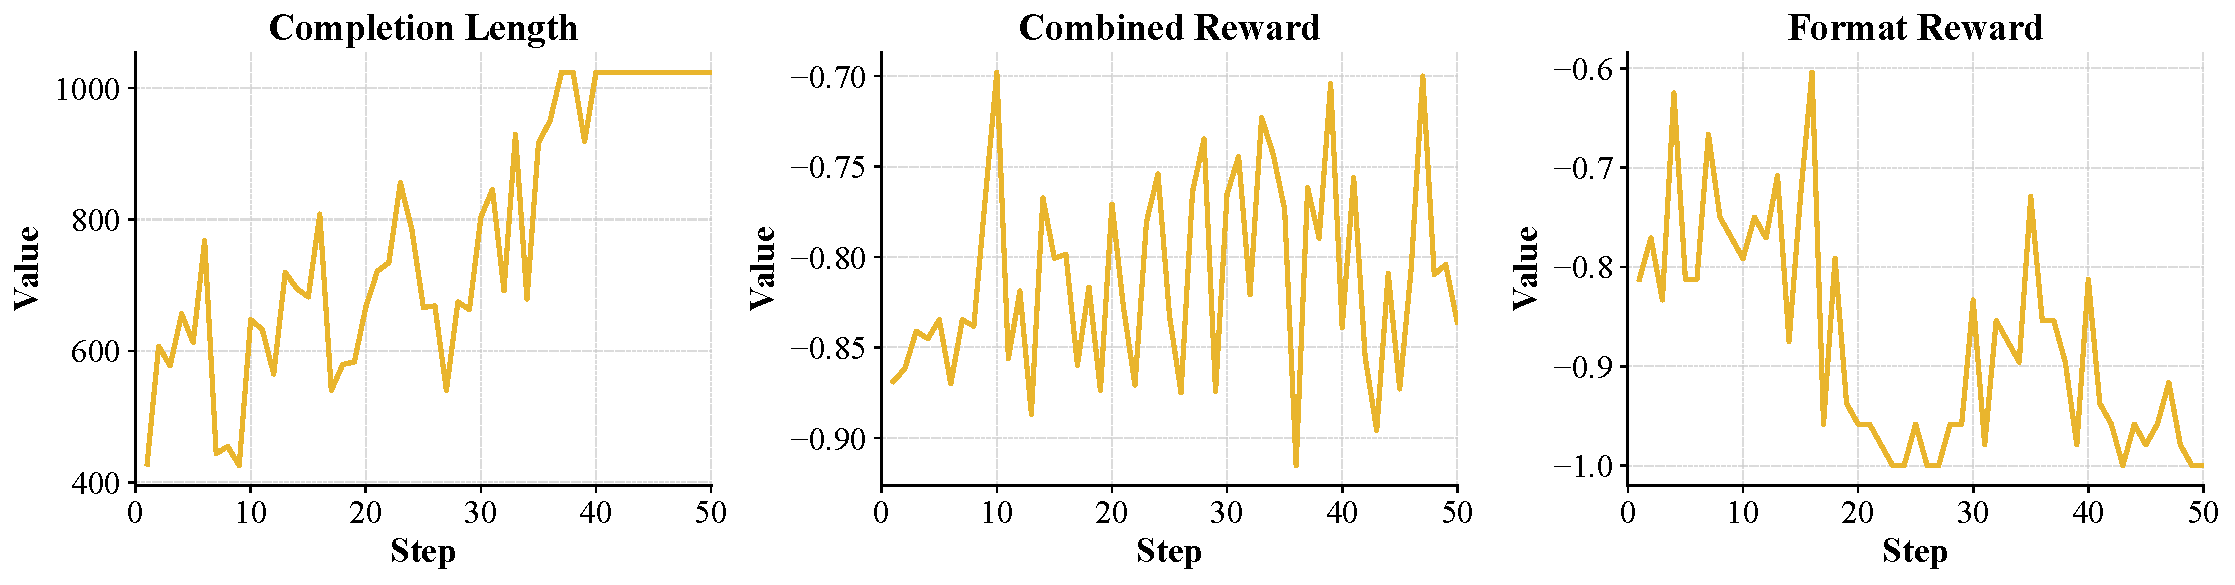
\includegraphics[width=0.95\linewidth]{images/rl-50steps.pdf}
%     \caption{DeepSeek-R1-Distill-Qwen-7B-ColdStart1200steps Training Curve.}
%     \label{ColdStart1200steps}
% \end{figure*}

% \newpage
% \section{Extended Evaluation on Reasoning Benchmarks}
% \label{appendix:extended-evaluation}
% To further demonstrate the robustness of our method on demanding reasoning tasks, we extend our evaluation beyond GPQA and AIME 2025 to include two additional challenging benchmarks: OlympiadBench and TheoremQA. These datasets test complex scientific and mathematical reasoning, requiring multi-step logical deduction far beyond simple Q\&A. The results reinforce our claim that KnowRL improves reasoning while mitigating hallucination.


% \subsection*{1. Performance on TheoremQA}
% \begin{table*}[h]
%     \small
%     %\setlength{\tabcolsep}{4pt}
%     \centering
%     \begin{tabular}{lccc}
%     \toprule
%     \textbf{Model} & \textbf{Direct Generation} & \textbf{KnowRL Trained} & \textbf{Improvement} \\
%     \midrule
%     DeepSeek-R1-Distill-Qwen-7B & 12.75\% & 17.88\% & +5.13\% \\
%     Skywork-OR1-7B-Preview    & 12.00\% & 15.12\% & +3.12\% \\
%     \bottomrule
%     \end{tabular}
%     \caption{Performance on TheoremQA.}
%     \label{tab:theoremqa}
% \end{table*}


% \subsection*{2. Performance on OlympiadBench}
% \begin{table*}[h]
%     \centering
%     \small
%     %\setlength{\tabcolsep}{4pt}
%     \begin{tabular}{lcccc}
%     \toprule
%     \textbf{Sub-task} & \textbf{DS-Base} & \textbf{DS-KnowRL} & \textbf{SW-Base} & \textbf{SW-KnowRL} \\
%     \midrule
%     maths\_en\_COMP      & 8.61\% & 9.94\% & 4.75\% & 7.42\% \\
%     maths\_zh\_COMP      & 7.35\% & 11.27\% & 5.39\% & 6.62\% \\
%     maths\_zh\_CEE       & 10.65\% & 9.35\% & 8.79\% & 8.15\% \\
%     physics\_en\_COMP    & 1.69\% & 1.27\% & 0.85\% & 0.00\% \\
%     physics\_zh\_CEE     & 7.83\% & 13.91\% & 3.48\% & 9.57\% \\
%     \bottomrule
%     \end{tabular}
%     \caption{Performance on OlympiadBench, with layout transposed for clarity. DS-Base: DeepSeek-R1-Distill-Qwen-7B, DS-KnowRL: the KnowRL-trained version. SW-Base: Skywork-OR1-7B-Preview, SW-KnowRL: the KnowRL-trained version.}
%     \label{tab:olympiadbench_transposed}
% \end{table*}

% On the TheoremQA benchmark, both the DeepSeek-R1-Distill-Qwen-7B and Skywork-OR1-7B-Preview models show significant accuracy improvements after being trained with KnowRL. On the more challenging OlympiadBench, the models trained with KnowRL exhibit only a slight performance decrease in the maths\_zh\_CEE and physics\_en\_COMP sub-tasks, while achieving considerable gains across the other tested math and physics categories. This demonstrates that KnowRL largely preserves and often enhances the models' complex reasoning capabilities.

% These new results, combined with our original findings on GPQA and AIME 2025, provide stronger evidence that our method successfully mitigates hallucination while simultaneously preserving and often enhancing the model's ability to tackle a wide array of complex, slow-thinking reasoning tasks.




%\newpage
% \section{Extended Evaluation on Diverse Model Architectures}
% \label{appendix:model-architectures}
% To test the generalizability of our framework, we extend our evaluation to two additional model types with distinct architectures: a slow-thinking model developed purely through Supervised Fine-Tuning (SFT) and a representative fast-thinking model.

% \begin{table*}[h]
% \centering
%     \small
%     %\setlength{\tabcolsep}{6pt}
%     \begin{tabular}{l|cc|cc}
%     \toprule
%     \multirow{3}{*}{\textbf{Benchmark}} & \multicolumn{2}{c|}{\textbf{OpenThinker3-7B (Slow)}} & \multicolumn{2}{c}{\textbf{Qwen2.5-7B-Instruct (Fast)}} \\
%     \cmidrule(lr){2-3} \cmidrule(lr){4-5}
%      & \textbf{Direct Generation} & \textbf{KnowRL} & \textbf{Direct Generation} & \textbf{KnowRL} \\
%     \midrule
%     TruthfulQA          & 38.19\% & 36.60\% & 30.97\% & 40.51\% \\
%     SimpleQA            & 3.55\%  & 7.61\%  & 4.09\%  & 3.29\%  \\
%     ChineseSimpleQA     & 15.67\% & 18.97\% & 29.00\% & 27.70\% \\
%     GPQA Diamond        & 28.28\% & 37.88\% & 35.86\% & 37.88\% \\
%     AIME2025            & 10.00\% & 20.00\% & 6.67\%  & 10.00\% \\
%     \bottomrule
%     \end{tabular}
%     \caption{Comparative performance of KnowRL on an SFT-based slow-thinking model (OpenThinker3-7B) and a fast-thinking model (Qwen2.5-7B-Instruct).}
%     \label{tab:Diverse_Model}
% \end{table*}

% As shown in Table~\ref{tab:Diverse_Model}, for the SFT-based slow-thinking model, OpenThinker3-7B, applying KnowRL yields substantial gains across both reasoning and factuality benchmarks. Performance on reasoning tasks like GPQA Diamond surges from 28.28\% to 37.88\%, and the score on AIME2025 doubles. Simultaneously, its factuality on datasets like SimpleQA and ChineseSimpleQA improves significantly.

% In contrast, the results on the fast-thinking model, Qwen2.5-7B-Instruct, are more nuanced. While the model's complex reasoning (AIME 2025) and truthfulness on a challenging dataset (TruthfulQA) improve after KnowRL training, its performance on simpler factual recall datasets (SimpleQA, ChineseSimpleQA) declines. This suggests a trade-off where imposing a deliberate, step-by-step reasoning process on a model optimized for rapid responses enhances complex logic at the cost of simple recall efficiency.

% In comparing these outcomes, it becomes clear that KnowRL's mechanism—rewarding a verifiable, step-by-step thinking process—aligns more naturally with the architecture of slow-thinking models, which is highly consistent with our paper's original motivation to solve the hallucination problem inherent to these models. Therefore, this comparative analysis leads us to a more refined conclusion: KnowRL is not as well-suited for trying to build up a model's reasoning skills and its ability to follow facts at the same time, from scratch. Rather, it is well-suited for models that are already good at 'slow thinking', as its primary role is to teach them how to reason based on facts while preserving their existing reasoning abilities.



\section{Case Analysis}
To explore KnowRL's impact on reasoning in factual tasks, we analyzed a reasoning case from the KnowRL training process, detailing the model's emergent reasoning behaviors. As shown in Figure~\ref{case}, these include Mixed-Language Reasoning, Knowledge Anchoring, Cross-verification, and Key Information Extraction. For simple factual tasks, distinct from mathematical reasoning, the model typically first proposes an initial answer (knowledge anchoring) and subsequently verifies this initial answer through reasoning behaviors such as reflection and cross-verification. This observed process aligns with human cognitive approaches when facing factual tasks, which further suggests the suitability of an outcome-based, reward-driven reinforcement learning training paradigm for open-domain factual tasks.

\begin{figure}[t]
    \centering
    \resizebox{0.48\textwidth}{!}{
    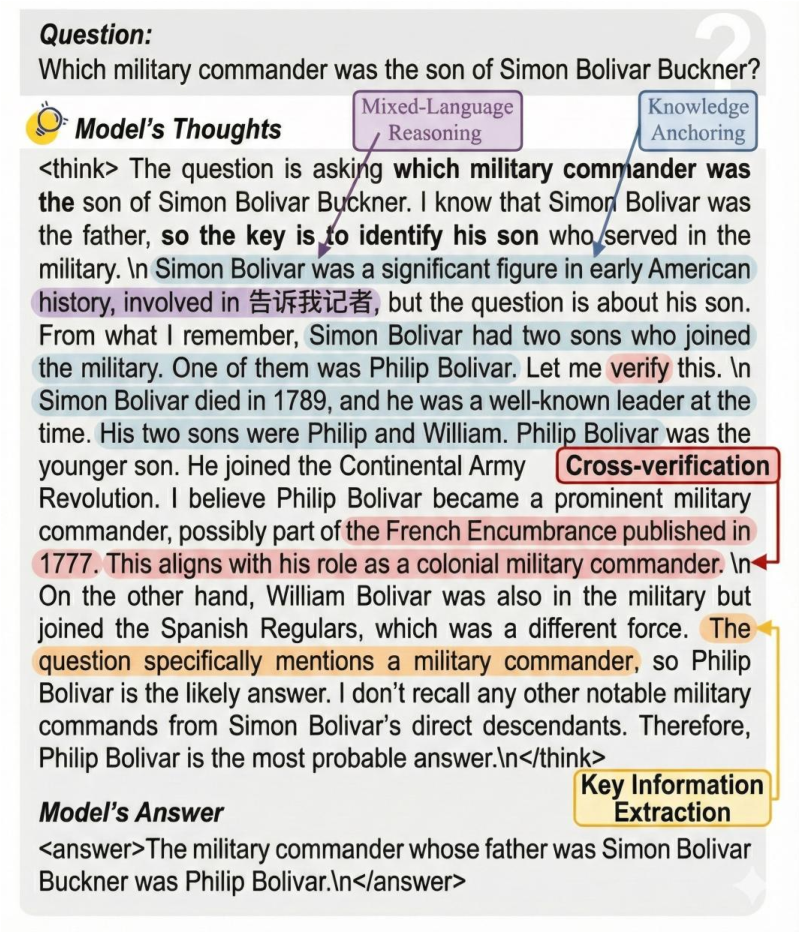
\includegraphics{images/new_case.pdf}}
    \caption{Case analysis of the KnowRL training process.}
    \vspace{-3ex}
     \label{case}
\end{figure}


\section{Training Dynamics of Different RL Algorithms}

\label{appendix:RL_algorithms}
As shown in Figure~\ref{fig:reward_comparison}, the reward curves for all four algorithms rise and stabilize, indicating successful convergence. 
Figure~\ref{fig:RL_algorithms} illustrates the training dynamics of the DeepSeek-R1-Distill-Qwen-7B model using BNPO, DAPO, and Dr.GRPO. A key observation is that all three algorithms effectively help the model establish clear knowledge boundaries to avoid hallucination. This effectiveness is evidenced by the rapid decline in completion length across all methods. The sharp drop indicates a behavioral shift where the model learns to provide concise refusals instead of generating long and potentially fabricated responses. This consistent pattern confirms that these RL approaches successfully guide the model toward reliable behavior and mitigate uncontrolled generation. Despite these shared trends, the algorithms differ in training efficiency and their impact on factual reasoning.



\begin{figure*}[t]
    \centering
    % --- 第一张图：BNPO ---
    \begin{subfigure}[b]{0.32\textwidth}
        \centering
        % 建议检查文件名：这里是 BNPO，但你之前的 caption 写的是 Skywork，请确认图片内容
        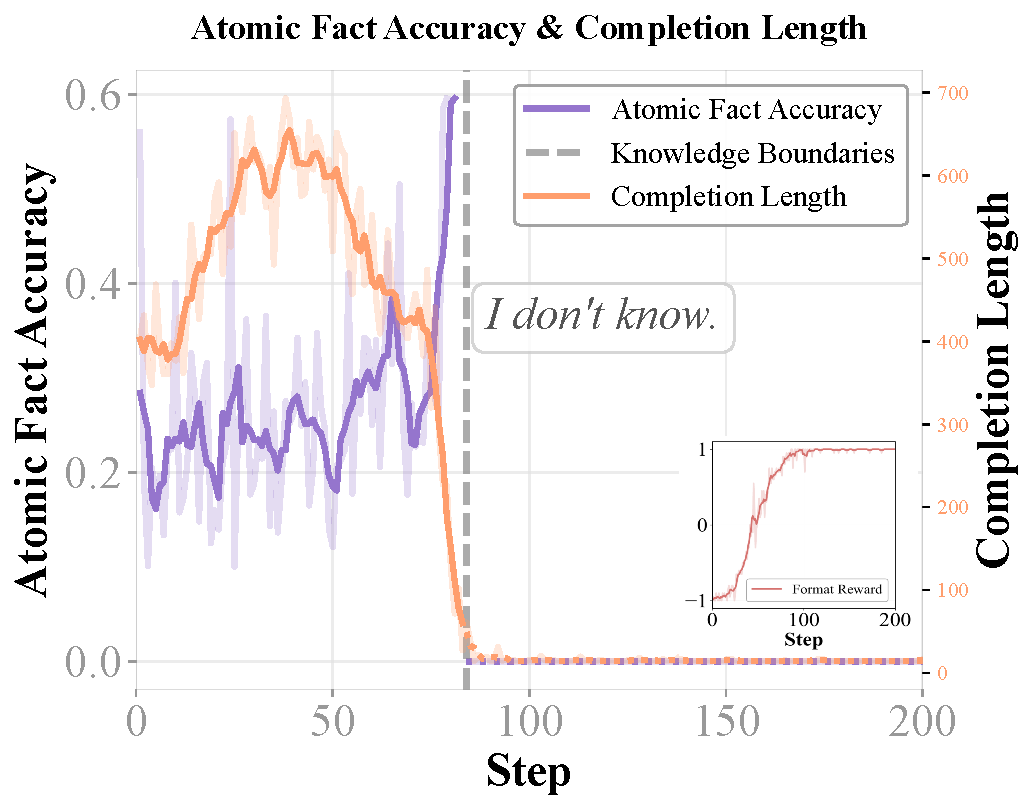
\includegraphics[width=\linewidth]{images/DeepSeek_BNPO.pdf}
        \caption{\textbf{BNPO}} 
        \label{fig:train_bnpo}
    \end{subfigure}
    \hfill % 弹性间距，让三张图撑满一行
    % --- 第二张图：DAPO ---
    \begin{subfigure}[b]{0.32\textwidth}
        \centering
        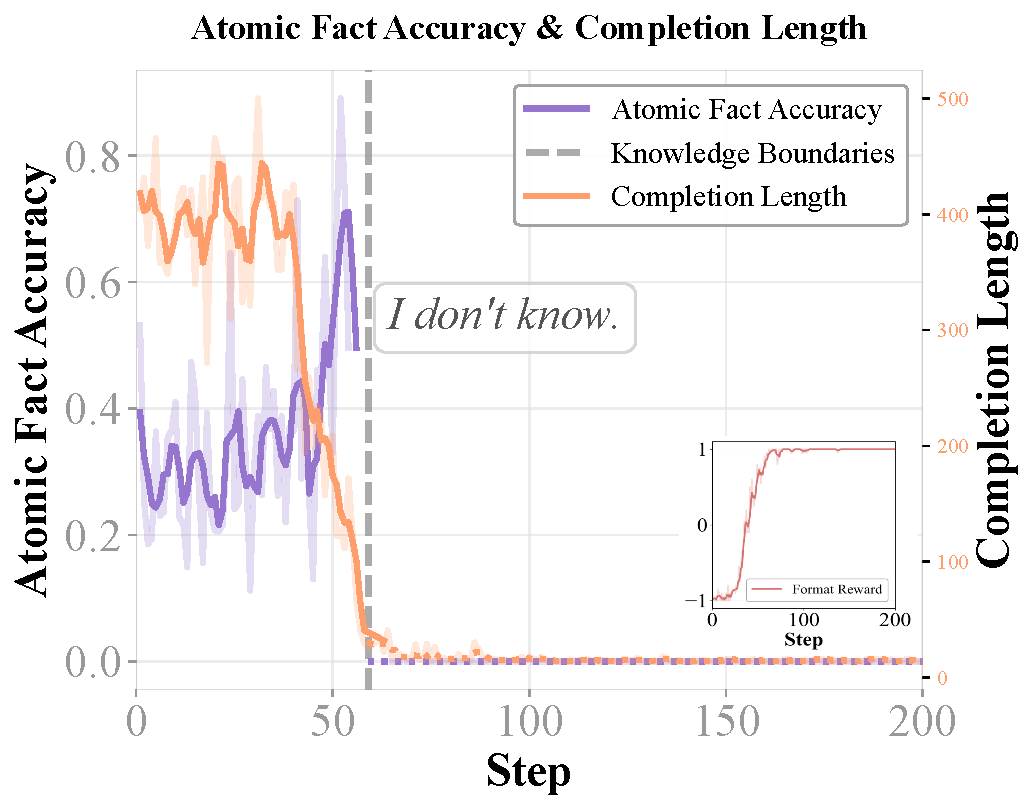
\includegraphics[width=\linewidth]{images/DeepSeek_DAPO.pdf}
        \caption{\textbf{DAPO}}
        \label{fig:train_dapo}
    \end{subfigure}
    \hfill
    % --- 第三张图：Dr.GRPO ---
    \begin{subfigure}[b]{0.32\textwidth}
        \centering
        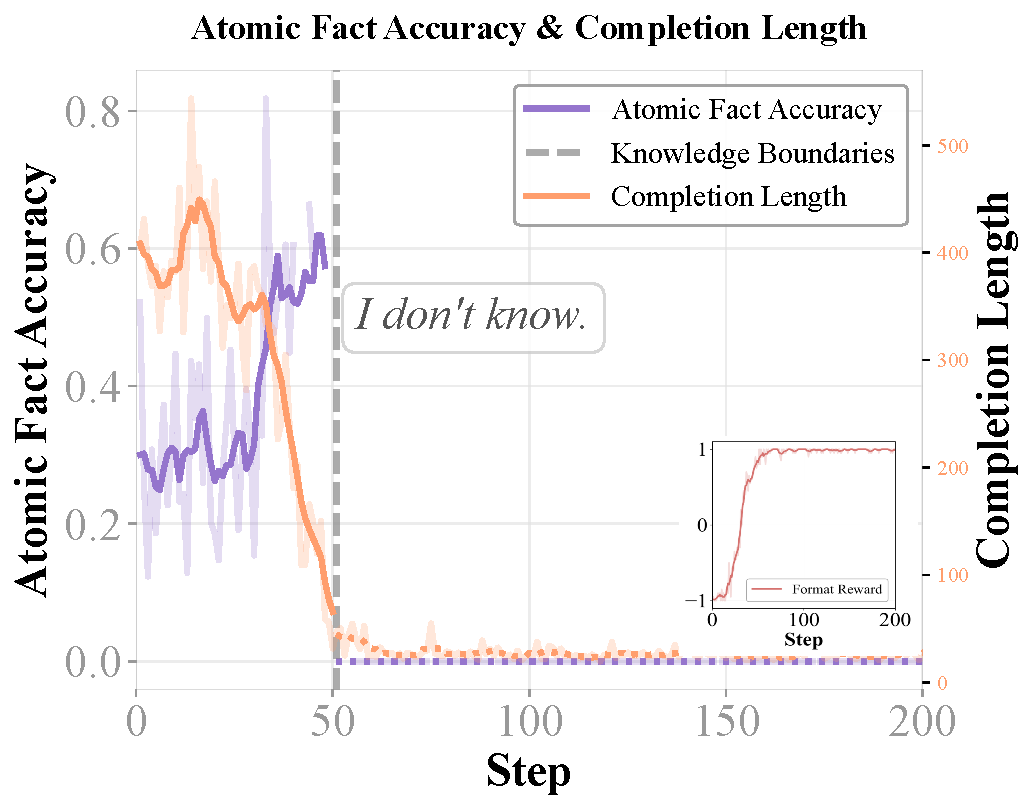
\includegraphics[width=\linewidth]{images/DeepSeek_DR.GRPO.pdf}
        \caption{\textbf{Dr.GRPO}}
        \label{fig:train_drgrpo}
    \end{subfigure}

    % --- 主标题：统一解释 ---
    \caption{
        \textbf{Training Dynamics on DeepSeek-R1-Distill-Qwen-7B.} 
        We visualize the training curves of different RL algorithms: (a) BNPO, (b) DAPO, and (c) Dr.GRPO. 
    }
    \vspace{-3ex} % 减少图片与正文的距离，节省版面
    \label{fig:RL_algorithms}
\end{figure*}




\section{Scalability Analysis on Larger Models}
\label{appendix:scalability}

We further evaluate the scalability of KnowRL by extending our experiments to the DeepSeek-R1-Distill-Qwen-14B model. As illustrated in Table~\ref{tab:perf_transposed}, KnowRL maintains its efficacy in mitigating hallucinations while simultaneously enhancing reasoning capabilities. Notably, on SimpleQA, our method significantly reduces the Incorrect Rate from 83.00\% to 68.33\% while doubling the Refusal Rate (13.33\% to 26.33\%). This shift indicates that the model acquires a more precise awareness of knowledge boundaries on larger architectures. Furthermore, KnowRL preserves and even strengthens complex reasoning performance, evidenced by the improvement in GPQA Diamond accuracy from 46.97\% to 51.01\%. These results validate that the benefits of our approach are robust and scalable across different model sizes.

\begin{figure}[h]
    \centering
    \resizebox{.425\textwidth}{!}{
    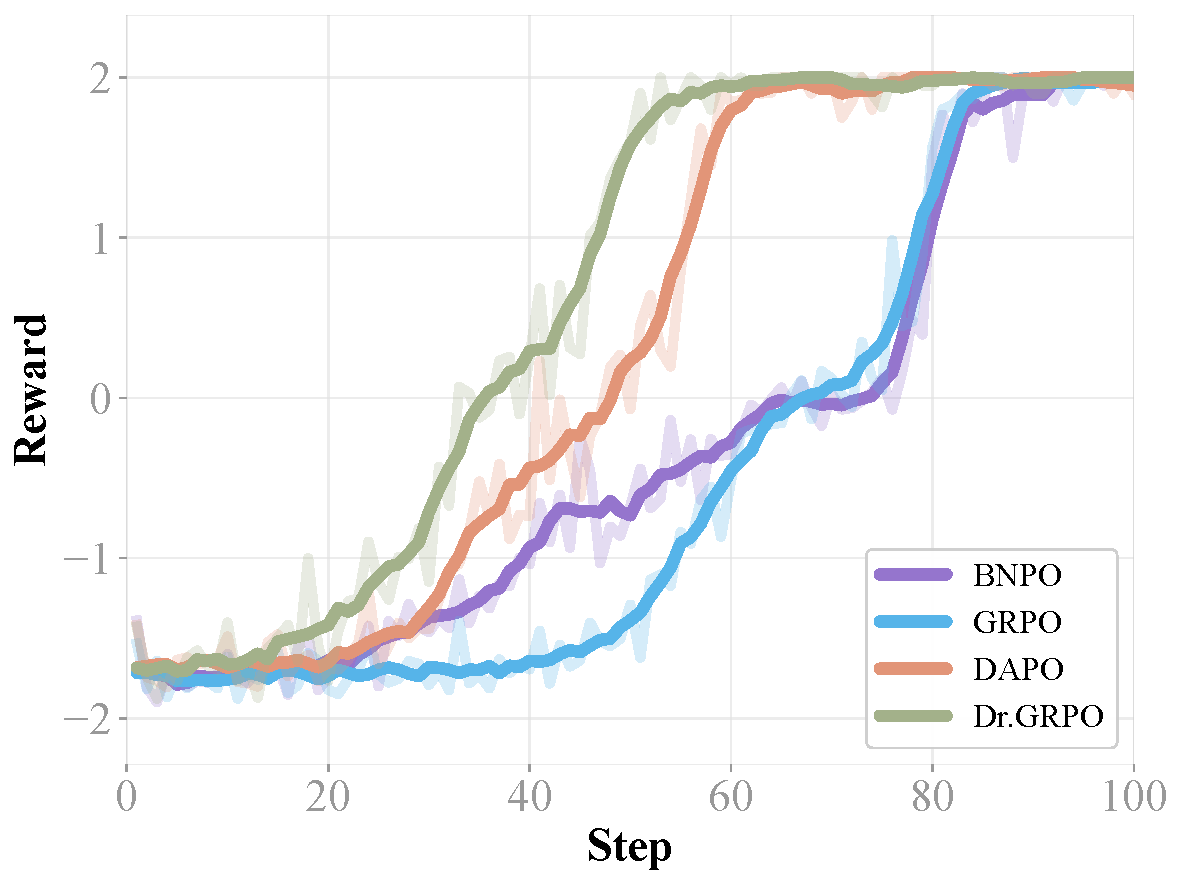
\includegraphics{images/combined_reward_comparison.pdf}}
    \caption{
    Comparison of training reward curves across different algorithms.}
    \vspace{-3ex}
    \label{fig:reward_comparison}
\end{figure}

\begin{table}[h]
    \centering
    \small
    \setlength{\tabcolsep}{13pt} % 稍微增加列间距，提升阅读舒适度
    \renewcommand{\arraystretch}{0.9} % 增加行高，避免拥挤
    \begin{tabular}{lcc}
    \toprule
    \textbf{Metric} & \textbf{Zero-shot} & \textbf{KnowRL} \\
    \midrule
    \multicolumn{3}{l}{\textit{TruthfulQA}} \\
    \quad Rouge & 53.33 & 54.67 \\
    \quad Bleu  & 50.33 & 55.00 \\
    \addlinespace[2pt] % 增加一点组间距
    \multicolumn{3}{l}{\textit{SimpleQA}} \\
    \quad PAQ & 4.23 & 6.17 \\
    \quad Incorrect & 83.00 & 68.33 \\
    \quad Refusal & 13.33 & 26.33 \\
    \quad F1 & 3.93 & 6.14 \\
    \addlinespace[3pt]
    \multicolumn{3}{l}{\textit{ChineseSimpleQA}} \\
    \quad PAQ & 29.18 & 31.07 \\
    \quad Incorrect & 63.33 & 61.33 \\
    \quad Refusal & 6.33 & 11.00 \\
    \quad F1 & 28.23 & 29.28 \\
    \addlinespace[3pt]
    \multicolumn{3}{l}{\textit{GPQA Diamond}} \\
    \quad Accuracy & 46.97 & 51.01 \\
    \addlinespace[3pt]
    \multicolumn{3}{l}{\textit{AIME}} \\
    \quad Accuracy & 40.00 & 36.67 \\
    \bottomrule
    \end{tabular}
    \caption{Performance comparison on DeepSeek-R1-Distill-Qwen-14B. The results demonstrate that KnowRL consistently improves hallucination mitigation (SimpleQA) and reasoning (GPQA) compared to the Zero-shot baseline.}
    \label{tab:perf_transposed}
\end{table}





\section{Evaluator Sensitivity Analysis}
\label{appendix:sensitivity}



\begin{table}[H]
    \centering
    \small
    \setlength{\tabcolsep}{5.5pt} % 增加列间距
    \renewcommand{\arraystretch}{0.9} % 增加行高
    \begin{tabular}{lcc}
    \toprule
    \textbf{Metric} & \textbf{Qwen2.5-72B-Instruct} & \textbf{GPT-4o-mini} \\
    \midrule
    \multicolumn{3}{l}{\textit{TruthfulQA}} \\
    \quad Rouge & 57.00 & 57.33 \\
    \quad Bleu  & 53.67 & 51.60 \\
    \addlinespace[2pt]
    \multicolumn{3}{l}{\textit{SimpleQA}} \\
    \quad PAQ & 1.53 & 2.81 \\
    \quad Incorrect & 64.33 & 57.67 \\
    \quad Refusal & 34.67 & 40.67 \\
    \quad F1 & 1.21 & 2.09 \\
    \addlinespace[3pt]
    \multicolumn{3}{l}{\textit{ChineseSimpleQA}} \\
    \quad PAQ & 9.74 & 10.26 \\
    \quad Incorrect & 58.67 & 58.33 \\
    \quad Refusal & 35.00 & 35.00 \\
    \quad F1 & 7.68 & 8.08 \\
    \addlinespace[3pt]
    \multicolumn{3}{l}{\textit{GPQA Diamond}} \\
    \quad Accuracy & 38.38 & 36.87 \\
    \addlinespace[3pt]
    \multicolumn{3}{l}{\textit{AIME}} \\
    \quad Accuracy & 33.33 & 33.33 \\
    \bottomrule
    \end{tabular}
    \caption{Robustness analysis of KnowRL using different evaluator models during training.}
    \label{tab:evaluator_comparison}
\end{table}

To confirm that the effectiveness of KnowRL is not dependent on a specific reward model used during training (e.g., GPT-4o-mini), we conducted an ablation study by replacing it with Qwen2.5-72B-Instruct \citep{qwen2.5}. 
As presented in Table~\ref{tab:evaluator_comparison}, the results demonstrate that KnowRL maintains comparable performance across different evaluators. 
Specifically, we observe that the model trained with GPT-4o-mini exhibits more conservative behavior, achieving a higher Refusal Rate and a lower Incorrect Rate on SimpleQA. In contrast, using Qwen2.5-72B-Instruct yields slightly higher performance on reasoning-heavy benchmarks like GPQA Diamond, suggesting a subtle trade-off between strict factuality enforcement and reasoning preservation depending on the evaluator's characteristics. 
This confirms that the efficacy of our method stems from the intrinsic KnowRL framework rather than reliance on a specific external judge.





\section{Evaluation of Generative Diversity}
\label{app:generative_diversity}

To investigate whether KnowRL's boundary-aware training inadvertently leads to over-conservatism or a loss of generative diversity, we evaluate our models using NoveltyBench \cite{zhang2025noveltybench}. This benchmark measures the ability of LLMs to produce diverse outputs for the same prompt. We conduct evaluations on the \textit{nb-curated} (100 prompts) and \textit{nb-wildchat} (1,000 prompts) subsets, sampling 10 responses per prompt at a temperature of 0.6. We report the \textit{distinct} metric, which averages the number of semantically unique equivalence classes across generations.

\begin{table}[h]
    \centering
    \small
    \setlength{\tabcolsep}{5.5pt} 
    \renewcommand{\arraystretch}{0.9} 
    \begin{tabular}{lcc}
    \toprule
    \textbf{Model} & \textbf{nb-curated} & \textbf{nb-wildchat} \\
    \midrule
    DeepSeek-7B & 1.61 & 1.71 \\
    DeepSeek-7B + KnowRL & 1.54 & 1.74 \\
    \midrule
    Skywork-7B & 1.63 & 1.65 \\
    Skywork-7B + KnowRL & 1.68 & 1.64 \\
    \bottomrule
    \end{tabular}
    \caption{Generative diversity (\textit{distinct} scores) on NoveltyBench subsets.}
    \label{tab:noveltybench}
\end{table}

As shown in Table \ref{tab:noveltybench}, the variation in \textit{distinct} scores after KnowRL training is extremely marginal ($\pm 0.01$ to $\pm 0.07$), indicating that the model's generative diversity remains intact. We attribute this preservation to the use of Low-Rank Adaptation (LoRA), which allows the model to learn new boundary-aware behaviors while mitigating the catastrophic forgetting of its original generative capabilities. While KnowRL increases refusal rates for out-of-knowledge queries to reduce hallucinations, it does not compromise the model's creative breadth in open-ended scenarios. We note that establishing an absolute ``False Refusal Rate'' remains challenging due to the difficulty of probing a model's precise internal knowledge, which we leave for future investigation.






\section{Implementation Details for Baselines}
\label{app:baseline_details}

To ensure fair comparison and reproducibility, all trainable baselines are fine-tuned using Low-Rank Adaptation (LoRA) and utilize the exact same QA training dataset as KnowRL.
The specific implementation details for each baseline are described as follows:

\begin{itemize}
    \item \textbf{Self-Refine (Prompt Engineering):} The model generates an initial response and then performs self-critique to provide feedback.
    It uses this self-feedback to refine its output iteratively.
    This ``FEEDBACK $\rightarrow$ REFINE'' loop is repeated until a stopping condition is met, specifically when it reaches a maximum of 5 iterations or when the model determines that no further improvement is needed.
    
    \item \textbf{SFT (Supervised Fine-Tuning):} We train the model using the correct reasoning processes and final answers distilled from the DeepSeek-R1 model as the target outputs.
    
    \item \textbf{DPO (Direct Preference Optimization):} We construct the preference pairs by using the correct answer distilled from DeepSeek-R1 as the ``chosen'' response, and the model's own incorrect generation as the ``rejected'' response.
    
    \item \textbf{FactTune-FS:} Following the methodology of the original paper \cite{REPLACE_WITH_FACTTUNE_CITATION}, we sample multiple responses from the model for a given prompt and evaluate them using FactScorer.
    We then construct DPO training pairs by selecting two responses that have a FactScore difference greater than 0.8.
    
    \item \textbf{TruthRL:} We adopt the exact same GRPO training setup as KnowRL to ensure a strictly fair comparison.
    We only change the reward function to match TruthRL's original design: $+1$ for a correct answer, $0$ for a refusal, and $-1$ for an incorrect answer.
\end{itemize}












%\onecolumn


\section{Prompts}

\label{appendix:4o-prompt}



\begin{tcolorbox}[breakable,title=Prompt Used by the GPT-4o for Data Filtering]

\columnseprule=0.5pt

You are an entity extraction assistant that identifies key entities in questions.





TASK:



1. First normalize the query by properly capitalizing names, titles, and other named entities



2. Determine if the query has sufficient context to be answered meaningfully



3. Extract only the most important entities from the query that are essential for answering it





RULES:



1. Extract a MAXIMUM of 2 specific entities (people, places, objects, works, etc.)



2. Output the MOST important entity first, then the secondary entity (if any)



3. Extract precise named entities, not general concepts or phrases



4. Keep related entities together as a single entity (e.g., character names with their roles)



5. Return individual entities rather than relationships or possessive forms



6. Only extract truly representative entities - ignore generic terms that don't specifically define the query



7. Only REJECT queries that meet the rejection criteria below



ONLY reject queries in these specific cases:



1. When the entity in the query is completely ambiguous (e.g., "Who is that person?")



2. When the query lacks necessary qualifying information (e.g., "Who will win?" with no mention of what contest)



3. When the query is too vague to determine its intent (e.g., "What happened to him?")



4. When the query is time-sensitive and contains temporal references like "now", "current", "latest", "recent", etc.



5. When the query lacks sufficient information to determine a single definitive answer, potentially leading to multiple correct interpretations or answers



6. Be careful not to extract purely numerical information such as a year as an entity





Note: Queries with historical context, pop culture references, geographical locations, or other well-defined entities should be ACCEPTED.





EXAMPLES:





Example 1:



Original Query: "who played barbara gordon batgirl?"



Normalized Query: "Who played Barbara Gordon Batgirl?"



Output: Normalized Query: "Who played Barbara Gordon Batgirl?"



      Entities: ["Barbara Gordon Batgirl"]

      

NOT: ["Barbara Gordon", "Batgirl"] - This is incorrect because "Barbara Gordon 

Batgirl" is a single character entity.



Example 2:



Original Query: "what continent does armenia belong to?"



Normalized Query: "What continent does Armenia belong to?"



Output: Normalized Query: "What continent does Armenia belong to?"



      Entities: ["Armenia"]

      

NOT: ["Armenia", "continent"] - The term "continent" is a generic category, not a specific entity representative of this query.





Example 3:



Original Query: "who is niall ferguson's wife?"



Normalized Query: "Who is Niall Ferguson's wife?"



Output: Normalized Query: "Who is Niall Ferguson's wife?"



      Entities: ["Niall Ferguson"]

      



Example 4:



Original Query: "who was the italian leader in ww1?"



Normalized Query: "Who was the Italian leader in WW1?"



Output: Normalized Query: "Who was the Italian leader in WW1?"



      Entities: ["Italian leader", "WW1"]



Example 5:



Original Query: "who will play mr gray in the film?"



Normalized Query: "Who will play Mr. Gray in the film?"



Output: Normalized Query: "Who will play Mr. Gray in the film?"



      REJECT (insufficient context - which film?)





Example 6:



Original Query: "who is in charge of libya now?"



Normalized Query: "Who is in charge of Libya now?"



Output: Normalized Query: "Who is in charge of Libya now?"



      REJECT (time-sensitive query with temporal reference "now")

      



Example 7:



Original Query: "what did werner heisenberg discover?"



Normalized Query: "What did Werner Heisenberg discover?"



Output: Normalized Query: "What did Werner Heisenberg discover?"



      REJECT (lacks sufficient specificity - Heisenberg made multiple discoveries)



Please try to output in this format:



Normalized Query: "The normalized version of the query"



Entities: ["entity1", "entity2"]



If you need to reject, still include the normalized query:



Normalized Query: "The normalized version of the query"



REJECT (reason for rejection)



Extract key entities from this query: "{query}"



\end{tcolorbox}



















\end{document}
